\documentclass[a4paper]{article}
\usepackage{vntex}
%\usepackage[english,vietnam]{babel}
%\usepackage[utf8]{inputenc}

%\usepackage[utf8]{inputenc}
%\usepackage[francais]{babel}
\usepackage{a4wide,amssymb,epsfig,latexsym,array,hhline,fancyhdr}
\usepackage[normalem]{ulem}
%\usepackage{soul}
\usepackage{caption}
\usepackage[makeroom]{cancel}
\usepackage{amsmath}
\usepackage{amsthm}
\usepackage{multicol,longtable,amscd}
\usepackage{diagbox}%Make diagonal lines in tables
\usepackage{booktabs}
\usepackage{alltt}
\usepackage[framemethod=tikz]{mdframed}% For highlighting paragraph backgrounds
\usepackage{caption,subcaption}
\usepackage{minted}
\usepackage{lastpage}
\usepackage[lined,boxed,commentsnumbered]{algorithm2e}
\usepackage{enumerate}
\usepackage{color}
\usepackage{graphicx}							% Standard graphics package
\usepackage{array}
\usepackage{tabularx, caption}
\usepackage{multirow}
\usepackage{multicol}
\usepackage{rotating}
\usepackage{graphics}
\usepackage{geometry}
\usepackage{setspace}
\usepackage{epsfig}
\usepackage{float}
\usepackage{tikz}
\usetikzlibrary{arrows,snakes,backgrounds}
\usepackage[unicode]{hyperref}
\hypersetup{urlcolor=blue,linkcolor=black,citecolor=black,colorlinks=true} 
%\usepackage{pstcol} 								% PSTricks with the standard color package
\usepackage{listings}
\lstset{
    language=Python,
    basicstyle=\ttfamily\small,
    keywordstyle=\color{blue},
    stringstyle=\color{red},
    commentstyle=\color{green},
    morecomment=[l][\color{magenta}]{\#},
    breaklines=true,
    postbreak=\mbox{\textcolor{red}{$\hookrightarrow$}\space},
}
\newcommand{\code}[1]{\texttt{\textcolor{blue!80!black}{#1}}}
\usepackage[normalem]{ulem}

\newtheorem{theorem}{{\bf Định lý}}
\newtheorem{property}{{\bf Tính chất}}
\newtheorem{proposition}{{\bf Mệnh đề}}
\newtheorem{corollary}[proposition]{{\bf Hệ quả}}
\newtheorem{lemma}[proposition]{{\bf Bổ đề}}
\theoremstyle{definition}
\newtheorem{exer}{Bài toán}

\def\thesislayout{	% A4: 210 × 297
	\geometry{
		a4paper,
		total={160mm,240mm},  % fix over page
		left=30mm,
		top=30mm,
	}
}
\thesislayout

%\usepackage{fancyhdr}
\setlength{\headheight}{40pt}
\pagestyle{fancy}
\fancyhead{} % clear all header fields
\fancyhead[L]{
 \begin{tabular}{rl}
    \begin{picture}(25,15)(0,0)
    \put(0,-8){
\includegraphics[width=8mm, height=8mm]{Images/hcmut.png}}
    %\put(0,-8){
\epsfig{width=10mm,figure=hcmut.eps}}
   \end{picture}&
	%
\includegraphics[width=8mm, height=8mm]{hcmut.png} & %
	\begin{tabular}{l}
		\textbf{\bf \ttfamily Trường Đại Học Bách Khoa Tp.Hồ Chí Minh}\\
		\textbf{\bf \ttfamily Khoa Khoa Học \& Kỹ Thuật Máy Tính}
	\end{tabular} 	
 \end{tabular}
}
\fancyhead[R]{
	\begin{tabular}{l}
		\tiny \bf \\
		\tiny \bf 
	\end{tabular}  }
\fancyfoot{} % clear all footer fields
\fancyfoot[L]{\scriptsize \ttfamily Bài tập lớn môn Học sâu và ứng dụng trong thị giác máy tính - Niên khóa 2025-2026}
\fancyfoot[R]{\scriptsize \ttfamily Trang {\thepage}/\pageref{LastPage}}
\renewcommand{\headrulewidth}{0.3pt}
\renewcommand{\footrulewidth}{0.3pt}


%%%
\setcounter{secnumdepth}{4}
\setcounter{tocdepth}{3}
\makeatletter
\newcounter {subsubsubsection}[subsubsection]
\renewcommand\thesubsubsubsection{\thesubsubsection .\arabic{subsubsubsection}}
\newcommand\subsubsubsection{\@startsection{subsubsubsection}{4}{\z@}%
                                     {-3.25ex\@plus -1ex \@minus -.2ex}%
                                     {1.5ex \@plus .2ex}%
                                     {\normalfont\normalsize\bfseries}}
\newcommand*\l@subsubsubsection{\@dottedtocline{3}{10.0em}{4.1em}}
\newcommand*{\subsubsubsectionmark}[1]{}
\makeatother

% \everymath{\color{blue}}%make in-line maths symbols blue to read/check easily

\sloppy
\captionsetup[figure]{labelfont={small,bf},textfont={small,it},belowskip=-1pt,aboveskip=-9pt}
%space remove between caption, figure, and text
\captionsetup[table]{labelfont={small,bf},textfont={small,it},belowskip=-1pt,aboveskip=7pt}
%space remove between caption, table, and text

%\floatplacement{figure}{H}%forced here float placement automatically for figures
%\floatplacement{table}{H}%forced here float placement automatically for table
%the following settings (11 lines) are to remove white space before or after the figures and tables
%\setcounter{topnumber}{2}
%\setcounter{bottomnumber}{2}
%\setcounter{totalnumber}{4}
%\renewcommand{\topfraction}{0.85}
%\renewcommand{\bottomfraction}{0.85}
%\renewcommand{\textfraction}{0.15}
%\renewcommand{\floatpagefraction}{0.8}
%\renewcommand{\textfraction}{0.1}
\setlength{\floatsep}{5pt plus 2pt minus 2pt}
\setlength{\textfloatsep}{5pt plus 2pt minus 2pt}
\setlength{\intextsep}{10pt plus 2pt minus 2pt}

\thesislayout

\begin{document}

\begin{titlepage}
	\begin{center}
		ĐẠI HỌC QUỐC GIA THÀNH PHỐ HỒ CHÍ MINH \\
		TRƯỜNG ĐẠI HỌC BÁCH KHOA \\
		KHOA KHOA HỌC \& KỸ THUẬT MÁY TÍNH
	\end{center}

	\vspace{1cm}

	\begin{figure}[h!]
		\begin{center}
			
\includegraphics[width=3cm]{Images/hcmut.png}
		\end{center}
	\end{figure}

	\vspace{1cm}


	\begin{center}
		\begin{tabular}{c}
			\multicolumn{1}{l}{\textbf{{\Large HỌC SÂU VÀ ỨNG DỤNG TRONG THỊ GIÁC MÁY TÍNH}}} \\
			~~                                                                                \\
			\hline
			\\
			\multicolumn{1}{l}{\textbf{{\large Đề bài tập lớn cho Nhóm 4}}}                   \\
			% \\
			% \textbf{{\Huge Thống kê mô tả và}} \\
			% \textbf{{\Huge Xác suất rời rạc với R}}\\
			\textbf{\Large Bài tập lớn số 1}                                                  \\
			% \textbf{\large môn Cấu trúc rời rạc}
			\\
			\hline
		\end{tabular}
	\end{center}

	\vspace{1.5cm}

	\begin{table}[h]
		\begin{tabular}{rrl}
			\hspace{5 cm} & GVHD:         & TS. Lê Thành Sách            \\

			              & SV thực hiện: & Nguyễn Hữu Trưởng - 2470573  \\
			              &               & Nguyễn Nhật Thanh - 2570316  \\
			              &               & Võ Thị Bích Phượng - 2470570 \\
		\end{tabular}
	\end{table}
	\vspace{1.5cm}
	\begin{center}
		\vfill
		{\footnotesize Tp. Hồ Chí Minh, Tháng 03/2026}
	\end{center}
\end{titlepage}


%\thispagestyle{empty}

\newpage
\tableofcontents
\newpage


\section{Giới thiệu đề tài}

\subsection{Ngữ cảnh và Mục tiêu}
Trong khuôn khổ môn học Học sâu và ứng dụng trong thị giác máy tính, nhóm chúng em thực hiện Bài tập lớn số 1 với chủ đề tập trung vào bài toán phân loại (classification). Mục tiêu cốt lõi của đề tài là vận dụng và đánh giá hiệu năng của các kiến trúc mạng nơ-ron học sâu tiên tiến trên ba loại dữ liệu khác biệt: ảnh, văn bản và đa phương thức (ảnh kết hợp văn bản).

Thông qua quá trình triển khai, nhóm hướng tới việc đạt được các mục tiêu cụ thể sau:
\begin{itemize}
	\item Chuẩn bị dữ liệu và thiết lập quy trình huấn luyện, đánh giá chuẩn xác.
	\item Vận dụng các mô hình pretrained đa dạng để giải quyết bài toán phân loại.
	\item So sánh, phân tích kết quả giữa các họ mô hình học sâu khác nhau thông qua bảng số liệu và biểu đồ trực quan.
\end{itemize}

\subsection{Phương pháp và Mô hình thực nghiệm}
Để thực hiện so sánh một cách toàn diện theo yêu cầu của Bài tập lớn, nhóm tiến hành xây dựng và huấn luyện (fine-tune) các mô hình sau:
\begin{itemize}
	\item \textbf{Với dữ liệu ảnh:} Đối chiếu hiệu năng giữa mạng tích chập truyền thống CNN (Convolutional Neural Networks) và kiến trúc ViT (Vision Transformer).
	\item \textbf{Với dữ liệu văn bản:} Đánh giá sự khác biệt giữa mạng nơ-ron hồi quy RNN (cụ thể là cấu trúc LSTM) và kiến trúc Transformer.
	\item \textbf{Với dữ liệu đa phương thức:} Khảo sát khả năng phân loại thông qua hai chiến lược tiếp cận là Zero-shot classification và Few-shot classification.
\end{itemize}

\subsection{Tập dữ liệu sử dụng}
Nhằm đảm bảo các mô hình được đánh giá một cách thuyết phục nhất, nhóm đã lựa chọn ba tập dữ liệu đáp ứng tiêu chí về độ phân biệt lớp và số lượng mẫu huấn luyện từ vài nghìn mẫu trở lên:
\begin{itemize}
	\item \textbf{Tập dữ liệu ảnh - CIFAR-10:} Đây là một trong những tập dữ liệu tiêu chuẩn và được gợi ý sử dụng cho bài toán phân loại ảnh.
	\item \textbf{Tập dữ liệu văn bản - IMDB:} Được lựa chọn cho tác vụ phân loại văn bản (text classification). \\
	\item \textbf{Tập dữ liệu đa phương thức - COCO-caption 2017:} Đây là tập dữ liệu cung cấp các cặp ảnh và văn bản thực sự, cùng mô tả một thực thể hoặc sự kiện, đáp ứng đúng yêu cầu của bài toán phân loại đa phương thức.
\end{itemize}
\subsubsection{Tập dữ liệu ảnh: CIFAR-10}
Tập dữ liệu CIFAR-10 bao gồm 60.000 ảnh màu có kích thước 32x32 pixel, được phân bổ đều vào 10 lớp vật thể và động vật khác nhau (như máy bay, ô tô, chó, mèo,...).

\begin{itemize}
	\item \textbf{Đáp ứng tiêu chí:} Tập dữ liệu có 50.000 ảnh dùng để huấn luyện, thỏa mãn hoàn toàn yêu cầu có từ vài nghìn mẫu trở lên (lớn hơn 5.000 mẫu). Đồng thời, với 10 lớp phân biệt, CIFAR-10 vượt mức tối thiểu 5 lớp mà đề bài bắt buộc.

	\item \textbf{Lý do lựa chọn:} Đây là một tập dữ liệu có độ khó vừa phải, các lớp có sự đa dạng về góc chụp và bối cảnh, khắc phục được sự đơn giản quá mức của tập MNIST. Điều này tạo ra một môi trường thử nghiệm hoàn hảo để nhóm đánh giá và so sánh năng lực trích xuất đặc trưng không gian của mạng tích chập (CNN) so với khả năng nắm bắt ngữ cảnh toàn cục của kiến trúc Vision Transformer (ViT).
\end{itemize}

\subsubsection{Tập dữ liệu văn bản: IMDB Movie Reviews}
Tập dữ liệu IMDB chứa 50.000 văn bản đánh giá phim tiếng Anh, với độ dài và cấu trúc ngữ nghĩa phong phú, đa dạng. Kích thước tập dữ liệu này hoàn toàn đáp ứng điều kiện về số lượng mẫu huấn luyện.

\begin{itemize}
	\item \textbf{Cách đáp ứng ràng buộc 5 lớp:} Thông thường, IMDB được dùng cho bài toán phân loại nhị phân (Tích cực/Tiêu cực). Tuy nhiên, vì đề bài quy định rõ bài toán nhị phân là không hợp lệ để so sánh mô hình và phải có ít nhất 5 lớp, nhóm đã tiến hành tiền xử lý (preprocessing) lại nhãn của tập dữ liệu. Dựa trên điểm số rating gốc của người dùng (từ 1 đến 10 sao), nhóm đã phân loại lại tập dữ liệu thành 5 lớp cảm xúc tương ứng (ví dụ: Rất tiêu cực, Tiêu cực, Trung lập, Tích cực, Rất tích cực).

	\item \textbf{Lý do lựa chọn:} Các đoạn đánh giá trên IMDB thường có cấu trúc câu dài và phức tạp. Việc phân loại thành 5 mức độ cảm xúc yêu cầu mô hình phải hiểu được các từ khóa nhấn mạnh và ngữ cảnh đảo ngược. Nhờ đó, nhóm có thể thấy rõ sự chênh lệch về hiệu năng khi xử lý chuỗi dài giữa mạng nơ-ron hồi quy RNN (LSTM) và cơ chế tự chú ý của Transformer.
\end{itemize}

\subsubsection{Tập dữ liệu đa phương thức: COCO Captions 2017}
COCO (Common Objects in Context) Captions là bộ dữ liệu tiêu chuẩn quy mô lớn dùng để nghiên cứu mối liên hệ giữa hình ảnh và ngôn ngữ tự nhiên.

\begin{itemize}
	\item \textbf{Đáp ứng tiêu chí:} Tập dữ liệu cung cấp các cặp ảnh - văn bản thực sự. Mỗi bức ảnh đi kèm với khoảng 5 câu mô tả (captions) do con người trực tiếp chú thích, đảm bảo sự liên kết chặt chẽ về mặt thực thể và sự kiện, tuân thủ tuyệt đối quy định không được phép ghép ảnh và văn bản một cách ngẫu nhiên. Đây cũng là một trong những tập dữ liệu được gợi ý trực tiếp trong hướng dẫn.

	\item \textbf{Lý do lựa chọn:} Sự đa dạng và độ phức tạp cao của COCO Captions cung cấp một nền tảng thử nghiệm lý tưởng để nhóm đánh giá sức mạnh của các mô hình đa phương thức. Cụ thể, nhóm sử dụng bộ dữ liệu này để đối chiếu hiệu quả của hai phương pháp tiếp cận: Zero-shot classification (khả năng mô hình nhận diện các lớp chưa từng thấy trong quá trình huấn luyện) và Few-shot classification (khả năng học nhanh từ một lượng rất nhỏ dữ liệu mẫu).
\end{itemize}

\subsection{Metric đánh giá (Evaluation Metrics)}

Để đảm bảo sự công bằng và khách quan khi đối chiếu kết quả giữa các kiến trúc mô hình khác nhau (CNN vs. ViT, RNN vs. Transformer), nhóm thống nhất sử dụng chung một hệ thống các độ đo (metrics).

\begin{itemize}
	\item \textbf{Accuracy (Độ chính xác toàn cục):} Đây là metric bắt buộc được sử dụng để đánh giá tổng quan tỷ lệ dự đoán đúng trên toàn bộ tập dữ liệu.
	      \begin{equation}
		      \text{Accuracy}=\frac{TP+TN}{TP+TN+FP+FN}
	      \end{equation}

	\item \textbf{F1-Score:} Trong các trường hợp các lớp dữ liệu có sự phân bổ không đồng đều (mất cân bằng lớp), F1-Score được bổ sung để đánh giá mô hình một cách toàn diện hơn, tránh sai lệch do độ chính xác ảo. F1-Score là trung bình điều hòa của Precision (Độ xác thực) và Recall (Độ bao phủ):
	      \begin{equation}
		      F1 = 2 \times \frac{\text{Precision} \times \text{Recall}}{\text{Precision} + \text{Recall}}
	      \end{equation}

	\item \textbf{Ma trận nhầm lẫn (Confusion Matrix):} Nhóm bổ sung thêm ma trận này nhằm trực quan hóa các trường hợp mô hình nhận diện sai, từ đó phục vụ cho việc phân tích lỗi sâu hơn ở phần sau.
\end{itemize}


\section{Giới thiệu về thuật toán CNN}\label{sec:dataset}

Trong bài toán OCR, Mạng Nơ-ron Tích chập (Convolutional Neural Network - CNN) không đơn thuần là một bộ phân loại (classifier) mà đóng vai trò là bộ mã hóa đặc trưng thị giác (\textit{Visual Feature Encoder}). Mục tiêu của nó là ánh xạ hình ảnh đầu vào $I \in \mathbb{R}^{H \times W \times C}$ (với $H, W, C$ lần lượt là chiều cao, chiều rộng và số kênh màu) thành một bản đồ đặc trưng (feature map) trừu tượng $X \in \mathbb{R}^{H' \times W' \times D}$.

\subsection{Động lực và ý tưởng cốt lõi}
Trước khi đi sâu vào kiến trúc, cần xem xét lý do CNN vượt trội hơn các mạng MLP (Multi-layer Perceptron) truyền thống trong xử lý ảnh:

\begin{enumerate}
	\item \textbf{Vấn đề bùng nổ tham số:} Nếu áp dụng MLP fully-connected trực tiếp lên một ảnh có kích thước lớn (ví dụ $1000 \times 1000$ pixels), số lượng trọng số sẽ tăng lên khổng lồ (lên tới $10^{12}$ cho một lớp ẩn), dẫn đến việc mô hình dễ bị \textit{overfitting} và tiêu tốn tài nguyên tính toán không cần thiết.
	\item \textbf{Cấu trúc không gian (Spatial Structure):} MLP coi các pixel là độc lập, trong khi hình ảnh có tính chất cục bộ (\textit{feature localization}) - các pixel lân cận có mối quan hệ mật thiết, và tính chất bất biến vị trí (\textit{translation invariance}) - một đặc trưng (như cạnh, góc) có ý nghĩa như nhau dù xuất hiện ở vị trí nào trong ảnh.
\end{enumerate}

Để giải quyết vấn đề này, CNN sử dụng ba cơ chế tính toán chính: \textbf{Local Receptive Fields} (Vùng cảm nhận cục bộ), \textbf{Shared Weights} (Chia sẻ trọng số) và \textbf{Spatial Subsampling} (Lấy mẫu không gian).
\begin{figure}[H]
	\centering
	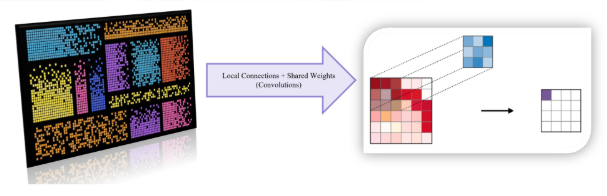
\includegraphics[width=1\linewidth]{Images/CNN_1.png}
	\vspace{10pt}
	\caption{Cơ chế tính toán của CNN}
	\label{fig:cnn-mechanism}
\end{figure}

\subsection{Các thành phần toán học và kiến trúc}

\subsubsection{Phép toán tích chập (Convolution Operation)}
Đây là lớp cốt lõi dùng để trích xuất các đặc trưng cục bộ. Thay vì kết nối đầy đủ, CNN sử dụng một bộ lọc (kernel/filter) $K$ có kích thước nhỏ $K_h \times K_w$ trượt qua toàn bộ ảnh.

Với một ảnh đầu vào $I$ và bộ lọc $K$, giá trị của bản đồ đặc trưng đầu ra $S$ tại vị trí $(i, j)$ được tính bằng công thức tích chập rời rạc:

\begin{equation}
	S(i, j) = (I * K)(i, j) = \sum_{u=0}^{K_h-1} \sum_{v=0}^{K_w-1} I(i - u, j - v) \cdot K(u, v)
\end{equation}

Ngoài ra, trong các ứng dụng thực tế như OCR, một lớp tích chập thường được biểu diễn dưới dạng:
\begin{equation}
	Y = \sigma(W * X + b)
\end{equation}
trong đó $W$ là kernel, $X$ là input, $b$ là bias, và $\sigma$ là hàm activation.

Ngoài kích thước bộ lọc, hai siêu tham số quan trọng kiểm soát kiến trúc là:
\begin{itemize}
	\item \textbf{Padding ($P$):} Thêm các pixel giả (thường là 0) xung quanh biên ảnh để kiểm soát kích thước đầu ra và tránh mất thông tin ở rìa ảnh.
	\item \textbf{Stride ($S$):} Bước nhảy của bộ lọc khi trượt trên ảnh. Stride càng lớn thì kích thước đầu ra càng nhỏ (giảm độ phân giải không gian).
\end{itemize}

Kích thước của Feature Map đầu ra ($H_{out} \times W_{out}$) được tính theo công thức:
\begin{equation}
	H_{out} = \left\lfloor \frac{H_{in} + 2P - K_h}{S} \right\rfloor + 1; \quad
	W_{out} = \left\lfloor \frac{W_{in} + 2P - K_w}{S} \right\rfloor + 1
\end{equation}

Trong ngữ cảnh OCR, các lớp tích chập đầu tiên sẽ học các đặc trưng cấp thấp (\textit{low-level features}) như các cạnh (edges), góc (corners). Các lớp sâu hơn sẽ tổ hợp lại để nhận diện các nét bút (strokes) và cấu trúc tô pô của ký tự.
\begin{figure}[H]
	\centering
	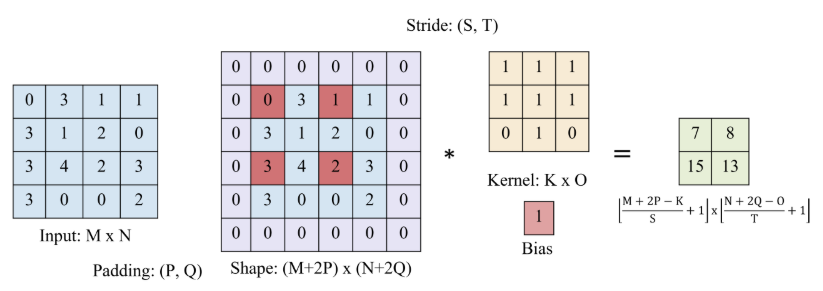
\includegraphics[width=0.95\linewidth]{Images/CNN_2.png}
	\vspace{10pt}
	\caption{Mô phỏng đơn giản về Convolution Layer}
	\label{fig:conv-layer}
\end{figure}

\subsubsection{Hàm kích hoạt phi tuyến (Non-linearity)}
Sau mỗi phép tích chập, một hàm kích hoạt phi tuyến được áp dụng để mô hình có thể học được các mối quan hệ phức tạp. Hàm phổ biến nhất là \textbf{ReLU (Rectified Linear Unit)}, giúp giảm thiểu vấn đề biến mất đạo hàm (\textit{vanishing gradient}) và tăng tốc độ hội tụ:

\begin{equation}
	f(x) = \max(0, x)
\end{equation}

Ngoài ReLU, có nhiều hàm activation khác được sử dụng trong các kiến trúc CNN hiện đại:

\begin{table}[h!]
	\centering
	\caption{So sánh các hàm Activation phổ biến}
	\begin{tabular}{|l|l|l|}
		\hline
		\textbf{Hàm Activation} & \textbf{Công thức}                                                         & \textbf{Ưu điểm/Nhược điểm}                           \\
		\hline
		ReLU                    & $f(x) = \max(0, x)$                                                        & Nhanh, tránh vanishing gradient, nhưng có dead neuron \\
		\hline
		Leaky ReLU              & $f(x) = \max(\alpha x, x)$                                                 & Khắc phục dead neuron của ReLU                        \\
		\hline
		ELU                     & $f(x) = \begin{cases} x & x > 0 \\ \alpha(e^x - 1) & x \leq 0 \end{cases}$ & Smooth, tốt hơn ReLU nhưng chậm hơn                   \\
		\hline
		Sigmoid                 & $f(x) = \frac{1}{1+e^{-x}}$                                                & Dễ hiểu nhưng dễ bị vanishing gradient                \\
		\hline
		Tanh                    & $f(x) = \frac{e^x - e^{-x}}{e^x + e^{-x}}$                                 & Đầu ra trong $[-1, 1]$, tốt hơn Sigmoid               \\
		\hline
	\end{tabular}
	\label{tab:activation}
\end{table}

\subsubsection{Pooling và Bất biến dịch chuyển}
Lớp Pooling thực hiện giảm chiều dữ liệu (\textit{down-sampling}) để giảm chi phí tính toán và tăng tính bất biến với các biến dạng nhẹ. Có hai loại phổ biến:
\begin{itemize}
	\item \textbf{Max Pooling:} Chọn giá trị lớn nhất trong vùng lân cận (giữ lại đặc trưng nổi bật nhất).
	      \begin{figure}[H]
		      \centering
		      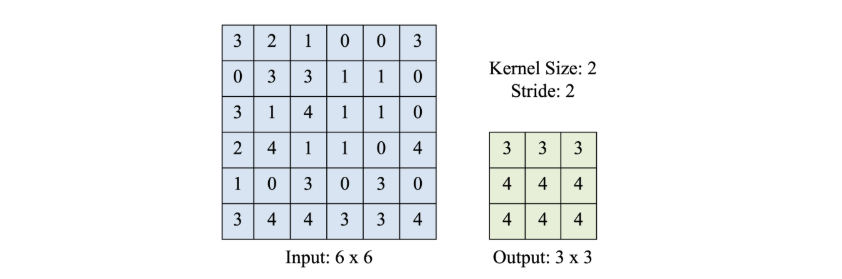
\includegraphics[width=0.95\linewidth]{Images/CNN_3.png}
		      \vspace{10pt}
		      \caption{Mô phỏng đơn giản về Max Pooling}
		      \label{fig:max-pooling}
	      \end{figure}
	\item \textbf{Average Pooling:} Tính giá trị trung bình trong vùng lân cận (làm mượt đặc trưng).
	      \begin{figure}[H]
		      \centering
		      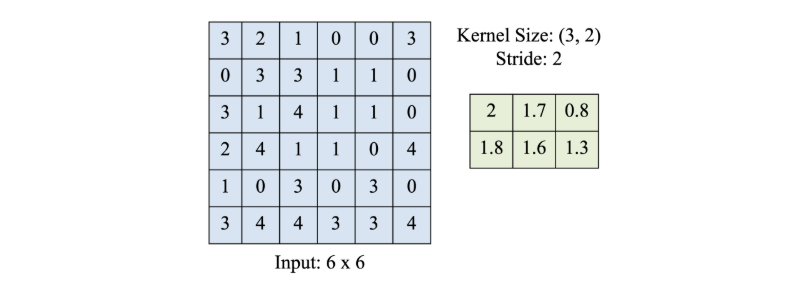
\includegraphics[width=0.95\linewidth]{Images/CNN_4.png}
		      \vspace{10pt}
		      \caption{Mô phỏng đơn giản về Average Pooling}
		      \label{fig:average-pooling}
	      \end{figure}
\end{itemize}

Về mặt toán học, với một vùng lân cận $R_{i,j}$ kích thước $K \times K$ và stride $S$, công thức tính kích thước đầu ra sau Pooling (không padding) là:
\begin{equation}
	H_{out} = \left\lfloor \frac{H_{in} - K}{S} \right\rfloor + 1
\end{equation}

Đối với OCR, lớp này giúp mô hình nhận diện được ký tự ngay cả khi nó bị dịch chuyển nhẹ hoặc co giãn trong ảnh (\textit{Translation Invariance}).

\begin{table}[H]
	\centering
	\caption{So sánh các loại Pooling}
	\begin{tabularx}{\textwidth}{|l|X|X|}
		\hline
		\textbf{Loại Pooling} & \textbf{Định nghĩa}                                             & \textbf{Ứng dụng}         \\
		\hline
		Max Pooling           & $y_{i,j} = \max_{(p,q) \in R_{i,j}} x_{p,q}$                    & Giữ lại feature mạnh nhất \\
		\hline
		Average Pooling       & $y_{i,j} = \frac{1}{|R_{i,j}|}\sum_{(p,q) \in R_{i,j}} x_{p,q}$ & Làm mịn features          \\
		\hline
		L2 Pooling            & $y_{i,j} = \sqrt{\sum_{(p,q) \in R_{i,j}} x_{p,q}^2}$           & Cân bằng hơn Max Pooling  \\
		\hline
	\end{tabularx}
	\label{tab:pooling}
\end{table}

\subsection{Mô hình hóa chuỗi (Sequence Modeling) với RNN}
Sau khi CNN trích xuất các đặc trưng hình ảnh, đầu ra là một chuỗi các vector đặc trưng $X = [x_1, x_2, ..., x_T]$, trong đó $T$ là chiều dài của chuỗi (tương ứng với chiều rộng của ảnh sau khi down-sampling). Tuy nhiên, CNN chỉ nắm bắt được thông tin cục bộ và thiếu khả năng xử lý ngữ cảnh chuỗi. Để giải quyết vấn đề này, Mạng Nơ-ron Hồi quy (RNN) được sử dụng.

\subsection{Hạn chế của RNN truyền thống và giải pháp LSTM}
Mạng RNN truyền thống cập nhật trạng thái ẩn $h_t$ dựa trên đầu vào hiện tại $x_t$ và trạng thái trước đó $h_{t-1}$:

\begin{equation}
	h_t = \tanh(W_{xh}x_t + W_{hh}h_{t-1} + b)
\end{equation}

Tuy nhiên, RNN thường gặp vấn đề \textit{biến mất đạo hàm} (vanishing gradient) khi xử lý các chuỗi dài, khiến nó không thể học được sự phụ thuộc xa. Để khắc phục, kiến trúc \textbf{Long Short-Term Memory (LSTM)} được đề xuất với cơ chế cổng (gating mechanism) bao gồm: cổng quên ($f_t$), cổng vào ($i_t$) và cổng ra ($o_t$), giúp điều tiết dòng thông tin qua các trạng thái tế bào ($c_t$).

\section{Phân loại văn bản với RNN \& Transformer}
\subsection{Tổng quan về Xử lý ngôn ngữ tự nhiên và Phân tích cảm xúc}
Xử lý Ngôn ngữ Tự nhiên (Natural Language Processing - NLP) là một nhánh của Trí tuệ Nhân tạo (AI) tập trung vào việc tương tác giữa máy tính và ngôn ngữ của con người. Trong giới hạn của nghiên cứu này, tác vụ cốt lõi được giải quyết là Phân tích cảm xúc (Sentiment Analysis) hay Phân loại văn bản (Text Classification).

Về mặt toán học, bài toán phân loại cảm xúc nhị phân có thể được định nghĩa như sau: Cho một tập hợp các văn bản (đánh giá phim) $D = \{d_1, d_2, \dots, d_N\}$ và tập nhãn phân lớp $Y = \{0, 1\}$, trong đó $0$ đại diện cho cảm xúc tiêu cực (Negative) và $1$ đại diện cho cảm xúc tích cực (Positive). Mục tiêu của mô hình học máy là tìm ra một hàm ánh xạ $f: D \rightarrow Y$ sao cho hàm mục tiêu (thường là sự sai lệch giữa dự đoán và thực tế) đạt giá trị nhỏ nhất.

\subsection{Cơ sở lý thuyết}

\subsubsection{Tiền xử lý dữ liệu và Không gian nhúng từ (Word Embeddings)}

\subsubsubsection{Tiền xử lý và Mã hóa (Tokenization)}
Máy tính không thể trực tiếp xử lý văn bản dạng chuỗi ký tự. Do đó, dữ liệu thô cần được làm sạch (loại bỏ nhiễu như thẻ HTML, ký tự đặc biệt) và phân rã thành các đơn vị cơ sở gọi là \textit{token} (từ, cụm từ, hoặc ký tự phụ). Mỗi token sau đó được ánh xạ thành một số nguyên duy nhất (ID) tạo thành một từ điển (Vocabulary). Tuy nhiên, việc biểu diễn bằng ID hay One-hot Encoding mang lại những ma trận thưa (sparse matrix) khổng lồ và hoàn toàn triệt tiêu mối quan hệ ngữ nghĩa giữa các từ.

\subsubsubsection{Biểu diễn từ phân tán với GloVe (Global Vectors for Word Representation)}
Để giải quyết hạn chế của One-hot Encoding, các kỹ thuật Word Embeddings ánh xạ mỗi từ vào một không gian vector thực liên tục (continuous vector space) nhiều chiều, nơi các từ có nghĩa tương đồng sẽ nằm gần nhau. Trong nghiên cứu này, thuật toán GloVe (cụ thể là ma trận GloVe 100 chiều) được sử dụng cho mô hình LSTM.

GloVe là một mô hình học không giám sát được phát triển bởi Đại học Stanford, kết hợp lợi thế của ma trận phân tích nhân tử toàn cục (global matrix factorization) và các phương pháp trượt cửa sổ ngữ cảnh cục bộ (local context window). Giả sử $X$ là ma trận đồng xuất hiện (co-occurrence matrix), trong đó phần tử $X_{ij}$ thể hiện số lần từ $j$ xuất hiện trong ngữ cảnh của từ $i$. Gọi $X_i = \sum_k X_{ik}$ là tổng số lần bất kỳ từ nào xuất hiện trong ngữ cảnh của $i$. Xác suất đồng xuất hiện được định nghĩa là $P_{ij} = P(j|i) = \frac{X_{ij}}{X_i}$.

GloVe thiết lập một hàm mục tiêu dựa trên bình phương sai số có trọng số (weighted least squares) nhằm tối thiểu hóa sự chênh lệch giữa tích vô hướng của hai vector nhúng và logarit xác suất đồng xuất hiện của chúng:
\begin{equation}
	J = \sum_{i,j=1}^{V} f(X_{ij}) \left( w_i^T \tilde{w}_j + b_i + \tilde{b}_j - \log X_{ij} \right)^2
\end{equation}
Trong đó:
\begin{itemize}
	\item $V$ là kích thước tập từ vựng.
	\item $w_i, \tilde{w}_j \in \mathbb{R}^d$ là các vector biểu diễn của từ mục tiêu và từ ngữ cảnh.
	\item $b_i, \tilde{b}_j$ là các hệ số chệch (bias).
	\item $f(X_{ij})$ là hàm trọng số nhằm giới hạn sự ảnh hưởng của các từ xuất hiện quá thường xuyên và ngăn chặn hàm $\log(0)$ khi $X_{ij} = 0$.
\end{itemize}

\subsubsection{Mạng Nơ-ron Hồi quy tiến hóa: Từ RNN đến Bi-LSTM}

\subsubsubsection{Mạng LSTM (Long Short-Term Memory)}
Mạng Nơ-ron Hồi quy (RNN) truyền thống gặp phải bài toán triệt tiêu đạo hàm (Vanishing Gradient) khi chuỗi quá dài. LSTM giải quyết vấn đề này thông qua kiến trúc tế bào (cell) phức tạp chứa "trạng thái ô" (cell state - $C_t$), cùng với ba "cổng" (gates) để kiểm soát luồng thông tin:

\begin{itemize}
	\item \textbf{Cổng quên (Forget gate - $f_t$):}
	      \begin{equation} f_t = \sigma(W_f \cdot [h_{t-1}, x_t] + b_f) \end{equation}
	\item \textbf{Cổng đầu vào (Input gate - $i_t$) và Trạng thái ứng viên ($\tilde{C}_t$):}
	      \begin{equation} i_t = \sigma(W_i \cdot [h_{t-1}, x_t] + b_i) \end{equation}
	      \begin{equation} \tilde{C}_t = \tanh(W_C \cdot [h_{t-1}, x_t] + b_C) \end{equation}
	\item \textbf{Cập nhật trạng thái ô ($C_t$):}
	      \begin{equation} C_t = f_t \odot C_{t-1} + i_t \odot \tilde{C}_t \end{equation}
	\item \textbf{Cổng đầu ra (Output gate - $o_t$) và Trạng thái ẩn ($h_t$):}
	      \begin{equation} o_t = \sigma(W_o \cdot [h_{t-1}, x_t] + b_o) \end{equation}
	      \begin{equation} h_t = o_t \odot \tanh(C_t) \end{equation}
\end{itemize}
\textit{(Trong đó: $\odot$ là ký hiệu cho phép nhân từng phần tử - element-wise multiplication).}

\begin{figure}[H]
	\centering
	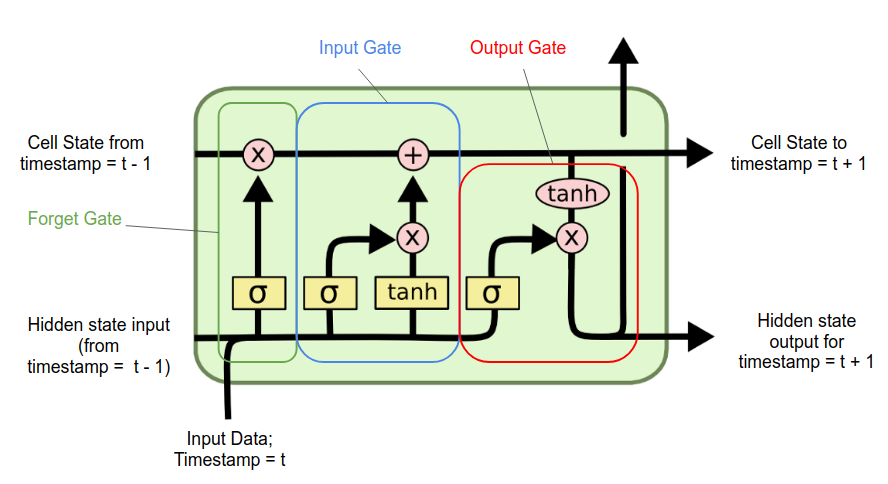
\includegraphics[width=0.75\linewidth]{Images/lstm.png}
	\vspace{10pt}
	\caption{Cấu trúc chi tiết của một tế bào LSTM (LSTM cell)}
	\label{fig:lstm}
\end{figure}

\subsubsubsection{Mạng LSTM hai chiều (Bidirectional LSTM) và Cơ chế Gộp (Pooling)}
Ngôn ngữ tự nhiên có tính phụ thuộc hai chiều. Bi-LSTM vận hành hai lớp LSTM song song: chiều xuôi ($\overrightarrow{h_t}$) và chiều ngược ($\overleftarrow{h_t}$). Trạng thái ẩn tổng hợp là sự ghép nối:
\begin{equation} h_t = [\overrightarrow{h_t} \oplus \overleftarrow{h_t}] \end{equation}

Để trích xuất đặc trưng toàn cục, mô hình sử dụng kết hợp hai phép toán Pooling:
\begin{itemize}
	\item \textbf{Average Pooling ($h_{avg}$):} Nắm bắt ngữ nghĩa tổng thể.
	\item \textbf{Max Pooling ($h_{max}$):} Phát hiện các từ khóa mang ý nghĩa quyết định.
\end{itemize}
Vector đặc trưng cuối cùng: $v_{out} = [h_{avg} \oplus h_{max}]$.

\subsubsection{Kiến trúc Transformer và Mô hình BERT}

\subsubsubsection{Cơ chế Tự chú ý (Self-Attention)}
Cơ chế này cho phép mô hình tính toán mức độ quan tâm của một từ đến tất cả các từ khác trong câu thông qua ba vector: Query ($Q$), Key ($K$) và Value ($V$):
\begin{equation}
	\text{Attention}(Q, K, V) = \text{softmax}\left(\frac{QK^T}{\sqrt{d_k}}\right)V
\end{equation}

\subsubsubsection{Mô hình BERT}
BERT (Bidirectional Encoder Representations from Transformers) dựa trên các khối Encoder của Transformer. Nghiên cứu áp dụng phiên bản \texttt{bert-base-uncased} (12 layers, hidden size 768). Đồ án sử dụng phương pháp Học chuyển giao (Transfer Learning) bằng cách Tinh chỉnh (Fine-tuning) lớp phân loại trên token đặc biệt \texttt{[CLS]}.

\begin{figure}[H]
	\centering
	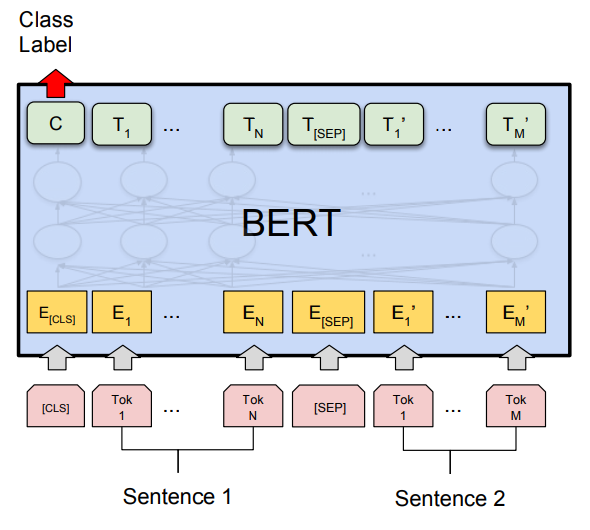
\includegraphics[width=0.6\linewidth]{Images/bert.png}
	\vspace{10pt}
	\caption{Khái quát kiến trúc mô hình BERT}
	\label{fig:bert}
\end{figure}

\subsubsection{Hàm mất mát và Kỹ thuật Tối ưu hóa}

\subsubsubsection{Hàm mất mát (Loss Functions)}
Đối với bài toán phân loại nhị phân, hàm Binary Cross-Entropy Loss được áp dụng:
\begin{equation}
	\mathcal{L}_{BCE} = -\frac{1}{N} \sum_{i=1}^N \left[ y_i \log(\sigma(\hat{y}_i)) + (1 - y_i) \log(1 - \sigma(\hat{y}_i)) \right]
\end{equation}

\subsubsubsection{Kỹ thuật chống Quá khớp (Overfitting)}
\begin{itemize}
	\item \textbf{Dropout:} Vô hiệu hóa ngẫu nhiên nơ-ron (tỷ lệ $p=0.3$).
	\item \textbf{Gradient Clipping:} Giới hạn $\text{max\_norm}=1.0$ để ngăn bùng nổ đạo hàm.
	\item \textbf{Tối ưu hóa:} Sử dụng thuật toán \textbf{AdamW} (cho BERT) và \textbf{Adam} (cho Bi-LSTM).
\end{itemize}

\subsubsection{Các độ đo đánh giá (Evaluation Metrics)}
Dựa trên ma trận nhầm lẫn (Confusion Matrix) với các giá trị $TP, TN, FP, FN$, các chỉ số được xác định như sau:

\begin{itemize}
	\item \textbf{Accuracy:} $\frac{TP + TN}{TP + TN + FP + FN}$
	\item \textbf{Precision:} $\frac{TP}{TP + FP}$
	\item \textbf{Recall:} $\frac{TP}{TP + FN}$
	\item \textbf{F1-Score:} $2 \times \frac{Precision \times Recall}{Precision + Recall}$
\end{itemize}

\subsection{Mô hình đề xuất}

Để giải quyết bài toán phân loại cảm xúc trên văn bản một cách hiệu quả, nghiên cứu này đề xuất và đối sánh hai quy trình hoàn chỉnh (end-to-end pipelines): một phương pháp dựa trên kiến trúc hồi quy truyền thống (Bi-LSTM kết hợp GloVe) và một phương pháp dựa trên học chuyển giao (Fine-tuning BERT). Chương này trình bày chi tiết về luồng xử lý dữ liệu, kiến trúc mạng nơ-ron và các chiến lược tối ưu hóa.

\subsubsection{Phân tích Khám phá và Phân chia Dữ liệu (EDA \& Data Splitting)}
Tập dữ liệu được sử dụng là \textit{IMDb Reviews Dataset}, bao gồm $50,000$ đánh giá điện ảnh được dán nhãn nhị phân. Tập dữ liệu thể hiện tính cân bằng hoàn hảo với tỷ lệ 50\% cho mỗi lớp (Tích cực và Tiêu cực), giúp loại bỏ rủi ro thiên lệch (class imbalance bias).

\begin{figure}[H]
	\centering
	\begin{minipage}{0.45\textwidth}
		\centering
		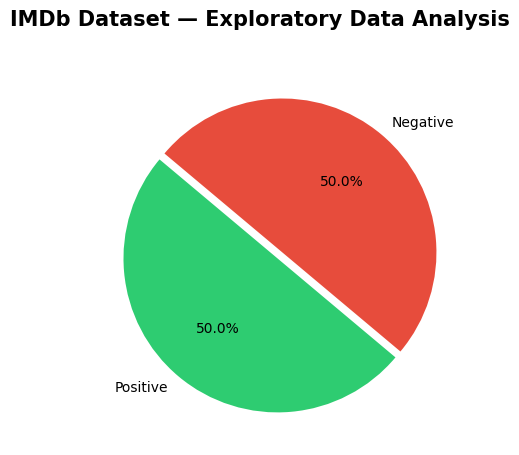
\includegraphics[width=\linewidth]{Images/imdb-1.png}
		\vspace{10pt}
		\caption{Phân phối nhãn tập dữ liệu}
		\label{fig:imdb-1}
	\end{minipage}\hfill
	\begin{minipage}{0.5\textwidth}
		\centering
		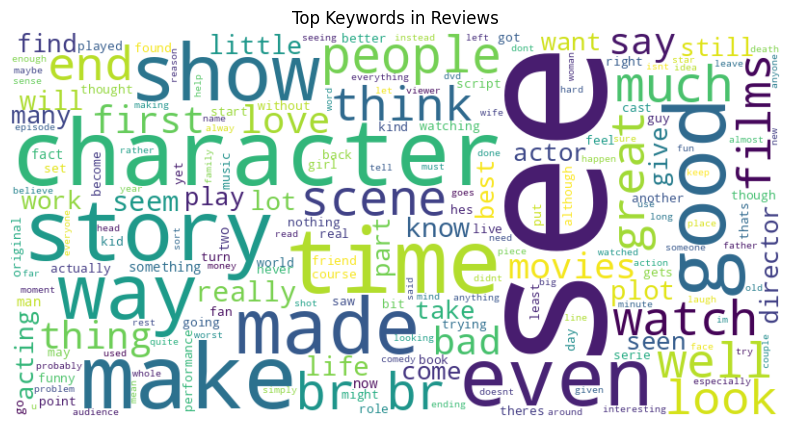
\includegraphics[width=\linewidth]{Images/imdb-word.png}
		\vspace{10pt}
		\caption{Từ khóa phổ biến trong các đánh giá}
		\label{fig:imdb-word}
	\end{minipage}
\end{figure}

Phân tích phân phối chỉ ra rằng 92.6\% số lượng đánh giá có độ dài $\le 512$ từ. Do đó, ngưỡng giới hạn chiều dài chuỗi (\textit{max sequence length}) được thiết lập như sau:

\begin{figure}[H]
	\centering
	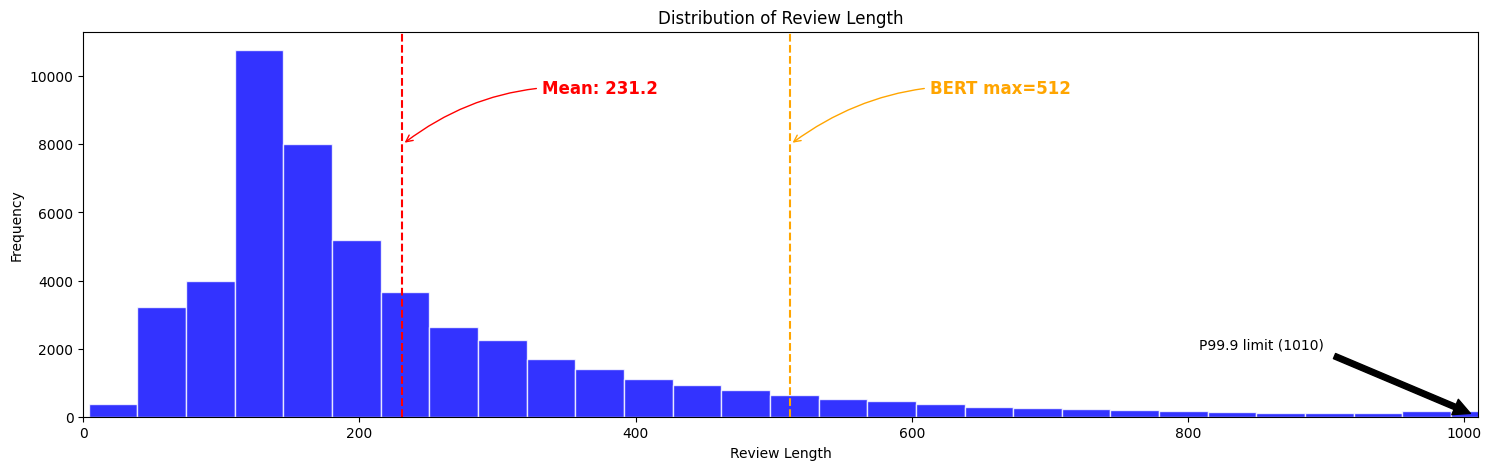
\includegraphics[width=0.95\linewidth]{Images/imdb-2.png}
	\vspace{10pt}
	\caption{Phân phối chiều dài các đánh giá trong tập dữ liệu}
	\label{fig:imdb-2}
\end{figure}

\begin{figure}[H]
	\centering
	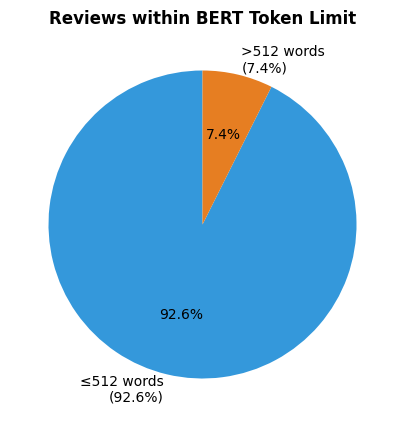
\includegraphics[width=0.5\linewidth]{Images/imdb-3.png}
	\vspace{10pt}
	\caption{Tỷ lệ đánh giá nằm trong giới hạn 512 từ của mô hình BERT}
	\label{fig:imdb-3}
\end{figure}
\begin{itemize}
	\item \textbf{Mô hình BERT:} 512 token (tối đa hóa ngữ nghĩa).
	\item \textbf{Mô hình Bi-LSTM:} 256 token (tối ưu hóa tốc độ tính toán).
\end{itemize}

Dữ liệu được phân chia theo chiến lược phân tầng (\textit{stratified split}) với tỷ lệ 80-10-10:
\begin{table}[h]
	\centering
	\begin{tabular}{|l|c|l|}
		\hline
		\textbf{Tập dữ liệu} & \textbf{Số lượng mẫu} & \textbf{Mục đích}                          \\ \hline
		Training Set         & $40,000$              & Cập nhật trọng số mạng.                    \\ \hline
		Validation Set       & $5,000$               & Tinh chỉnh siêu tham số và lưu checkpoint. \\ \hline
		Test Set             & $5,000$               & Đánh giá độ tổng quát hóa cuối cùng.       \\ \hline
	\end{tabular}
	\caption{Phân chia tập dữ liệu nghiên cứu}
\end{table}

\subsubsection{Tiền xử lý Văn bản và Biểu diễn Dữ liệu}
Nghiên cứu xây dựng quy trình chuẩn hóa văn bản thông qua hàm \texttt{clean\_text} sử dụng biểu thức chính quy (Regex) để: chuyển chữ thường, loại bỏ thẻ HTML (ví dụ: \texttt{<br />}), tách dấu câu và chuẩn hóa khoảng trắng.

\subsubsubsection{Biểu diễn cho mô hình Bi-LSTM}
Văn bản được tách từ dựa trên khoảng trắng và ánh xạ vào ma trận nhúng \textbf{GloVe 100 chiều} (\texttt{glove.6B.100d.txt}).
\begin{itemize}
	\item Kích thước từ vựng thực tế: $111,798$ token.
	\item Tỷ lệ bao phủ (\textit{Coverage}): 66.40\%.
	\item Các chuỗi ngắn hơn 256 được đệm (\textit{padding}) bằng ID 0.
\end{itemize}

\subsubsubsection{Biểu diễn cho mô hình BERT}
Sử dụng bộ \texttt{BertTokenizer} từ kiến trúc \texttt{bert-base-uncased} với thuật toán \textbf{WordPiece}. Kích thước từ vựng đạt $30,522$ token. Các chuỗi được xử lý tự động để đạt độ dài cố định \texttt{MAX\_LEN = 512}.

\subsubsection{Kiến trúc Đề xuất 1: Mạng Bi-LSTM tích hợp Gộp đặc trưng (Pooling)}
Mô hình \texttt{LSTMClassifier} bao gồm các tầng chức năng sau:

\begin{enumerate}
	\item \textbf{Embedding Layer:} Nhận đầu vào kích thước $(B \times 256)$, ánh xạ qua trọng số GloVe đã được đóng băng (\texttt{freeze=True}).
	\item \textbf{Bi-LSTM Layer:} Kích thước trạng thái ẩn (\textit{hidden size}) là $128$. Đầu ra tại mỗi bước thời gian $t$ là $h_t \in \mathbb{R}^{256}$ (do kết hợp hai chiều).
	\item \textbf{Multi-pooling Strategy:} Trích xuất đặc trưng toàn cục bằng cách nối kết (\textit{concatenate}) kết quả của Average Pooling và Max Pooling:
	      \begin{equation}
		      v_{concat} = \left[ \frac{1}{L} \sum_{t=1}^{L} h_t \right] \oplus \left[ \max_{t=1}^{L} h_t \right]
	      \end{equation}
	      Kết quả thu được vector đặc trưng $512$ chiều.
	\item \textbf{Classification Head:} Đi qua lớp Dropout ($p=0.3$) và một tầng tuyến tính (\texttt{nn.Linear(512, 1)}).
\end{enumerate}



\subsubsection{Kiến trúc Đề xuất 2: Tinh chỉnh Mô hình BERT (Fine-tuning)}
Nghiên cứu sử dụng biến thể \texttt{bert-base-uncased} (12 layers, 12 heads, 768 hidden size). Chiến lược \textbf{Học chuyển giao} được thực hiện bằng cách thêm một lớp phân loại tuyến tính lên trên token đầu ra \texttt{[CLS]}. Toàn bộ 109 triệu tham số sẽ được cập nhật nhẹ trong quá trình Fine-tuning.



\subsubsection{Cấu hình Huấn luyện và Chiến lược Tối ưu hóa}

\subsubsubsection{Tối ưu hóa Mô hình Bi-LSTM}
\begin{itemize}
	\item \textbf{Hàm mất mát:} Binary Cross Entropy with Logits.
	\item \textbf{Optimizer:} Adam ($\eta = 10^{-3}$).
	\item \textbf{Batch size:} 16; \textbf{Epochs:} 100.
	\item \textbf{Gradient Clipping:} \texttt{max\_norm=1.0}.
\end{itemize}

\subsubsubsection{Tối ưu hóa Mô hình BERT}
Quá trình Fine-tuning áp dụng các kỹ thuật đặc thù:
\begin{itemize}
	\item \textbf{Optimizer:} AdamW ($\eta = 2 \times 10^{-5}$, $\lambda = 0.01$).
	\item \textbf{Scheduler:} \textit{Linear Schedule with Warmup}. Tốc độ học tăng dần trong 10\% số bước đầu tiên (\textit{warmup ratio} = 0.1) sau đó giảm dần về 0.
	\item \textbf{Quy mô:} 3 epoch (tương đương 7,500 bước huấn luyện).
\end{itemize}



\subsubsubsection{Tóm tắt siêu tham số thực nghiệm}
\begin{table}[h]
	\centering
	\begin{tabular}{|l|c|c|}
		\hline
		\textbf{Thông số} & \textbf{Bi-LSTM + GloVe} & \textbf{BERT (Fine-tuning)} \\ \hline
		Learning Rate     & $10^{-3}$                & $2 \times 10^{-5}$          \\ \hline
		Optimizer         & Adam                     & AdamW                       \\ \hline
		Max Length        & 256                      & 512                         \\ \hline
		Batch Size        & 16                       & 16                          \\ \hline
		Epochs            & 100 (Early Stopping)     & 3                           \\ \hline
	\end{tabular}
	\caption{So sánh cấu hình huấn luyện của hai mô hình}
\end{table}

\subsection{Kết quả Thực nghiệm và Đánh giá}

Phần này trình bày chi tiết các kết quả đạt được sau quá trình huấn luyện hai kiến trúc mạng học sâu: Bi-LSTM kết hợp không gian nhúng GloVe và mô hình ngôn ngữ lớn BERT. Các phân tích được thực hiện dựa trên sự biến thiên của hàm mất mát, các độ đo phân loại chuẩn mực trên tập kiểm thử (Test Set) và đánh giá định tính qua các ca kiểm thử thực tế (Inference).

\subsubsection{Môi trường Thực nghiệm và Cấu hình Siêu tham số}
Nhằm đảm bảo tính công bằng và khả năng tái lập kết quả (reproducibility), toàn bộ các thực nghiệm được tiến hành trên cùng một môi trường phần cứng và phần mềm:
\begin{itemize}
	\item \textbf{Tài nguyên điện toán:} Bộ xử lý đồ họa (GPU) Tesla T4 với dung lượng bộ nhớ khả dụng xấp xỉ $15.6\text{ GB}$.
	\item \textbf{Cấu hình BERT:} Sử dụng biến thể \texttt{bert-base-uncased}. Thuật toán tối ưu AdamW được áp dụng với tốc độ học $\eta = 2 \times 10^{-5}$, hệ số suy giảm trọng số (weight decay) $0.01$ và tỷ lệ hâm nóng (warmup ratio) $0.1$. Quy mô lô (batch size) là 16. Quá trình tinh chỉnh (fine-tuning) diễn ra trong 3 epoch (tương đương 7,500 bước huấn luyện).
	\item \textbf{Cấu hình Bi-LSTM:} Đầu vào được giới hạn 256 token, đi qua ma trận nhúng GloVe 100 chiều. Thuật toán tối ưu Adam với $\eta = 10^{-3}$, batch size 16. Quá trình huấn luyện được thiết lập chạy tối đa 100 epoch để quan sát rõ ranh giới hội tụ và quá khớp.
\end{itemize}

\subsubsection{Phân tích Động lực học Quá trình Huấn luyện}
Sự biến thiên của hàm suy hao (Loss) và độ chính xác (Accuracy) qua các kỷ nguyên là cơ sở để đánh giá khả năng tổng quát hóa của mô hình.

\subsubsubsection{Động lực học của Mô hình BERT}
Quá trình tinh chỉnh BERT cho thấy sự hội tụ cực kỳ nhanh chóng. Ngay tại Kỷ nguyên 1 (Epoch 1), hàm mất mát trên tập huấn luyện (Train Loss) đã giảm xuống mức $0.2669$, đồng thời độ chính xác (Train Acc) đạt $89.35\%$. Tương ứng, độ chính xác trên tập kiểm định (Validation) đạt $93.22\%$.

Tuy nhiên, biểu đồ huấn luyện cho thấy dấu hiệu của hiện tượng quá khớp vi mô (micro-overfitting) bắt đầu xuất hiện từ Kỷ nguyên 2:
\begin{itemize}
	\item Train Loss tiếp tục giảm mạnh xuống $0.0744$ và Train Acc đạt đỉnh $98.16\%$.
	\item Ngược lại, Validation Loss bắt đầu tăng ngược trở lại lên mức $0.2696$, dù Validation Acc vẫn cải thiện nhẹ lên $93.88\%$.
\end{itemize}
Hệ thống đã tự động lưu lại điểm kiểm tra (checkpoint) tại Kỷ nguyên 2 với chỉ số $Best\ Val\ F1 = 0.9388$ làm mô hình dự đoán chính thức.

\begin{figure}[H]
	\centering
	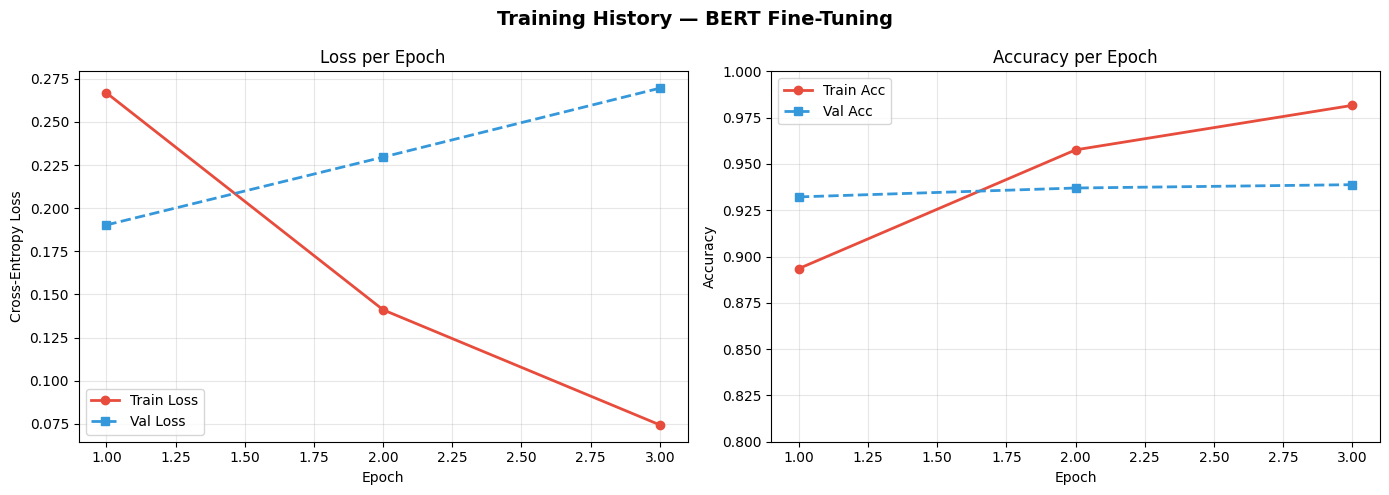
\includegraphics[width=\linewidth]{Images/bert-training.png}
	\vspace{10pt}
	\caption{Đồ thị hàm mất mát và độ chính xác của mô hình BERT qua 3 epoch}
	\label{fig:bert-training}
\end{figure}

\subsubsubsection{Động lực học của Mô hình Bi-LSTM}
Trái ngược với khả năng hội tụ ổn định của BERT, Bi-LSTM bộc lộ rõ rệt đặc tính khó kiểm soát của mạng hồi quy khi đối mặt với dữ liệu nhiễu trong thời gian dài.
\begin{itemize}
	\item Xuyên suốt 100 kỷ nguyên, Train Loss của LSTM tiệm cận về 0 (đạt $0.0146$ ở Epoch 100) và Train Acc gần như hoàn hảo ở mức $99.62\%$.
	\item Dẫu vậy, bắt đầu từ khoảng Epoch 10-15, Validation Loss bắt đầu phân kỳ và tăng theo cấp số nhân, đạt mức $1.3039$ ở Epoch cuối cùng, kéo theo Validation Acc suy giảm xuống $88.90\%$.
\end{itemize}
Sự phân kỳ sâu sắc này là minh chứng toán học kinh điển cho hiện tượng quá khớp (Overfitting) nghiêm trọng. Mạng LSTM, do hạn chế về dung lượng bộ nhớ ngữ cảnh xa, đã chọn cách "học vẹt" các đặc trưng cục bộ của tập huấn luyện thay vì rút ra quy luật ngôn ngữ tổng quát. Điểm $Best\ Val\ F1$ tối ưu nhất được ghi nhận là $0.8994$ trước khi mô hình trượt dài vào vùng quá khớp.

\begin{figure}[H]
	\centering
	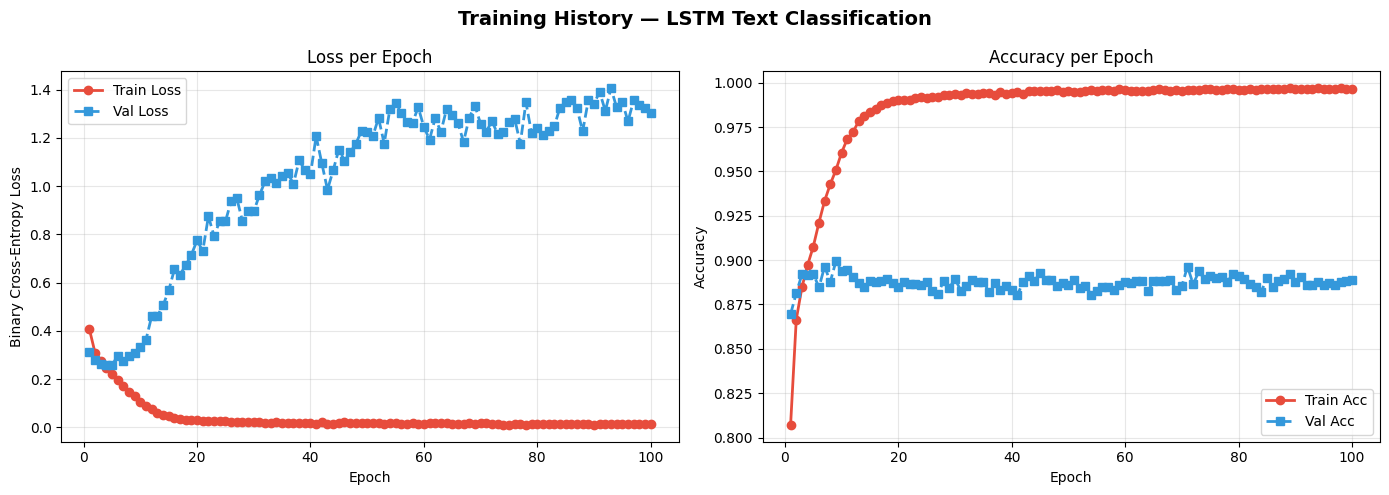
\includegraphics[width=\linewidth]{Images/lstm-training.png}
	\vspace{10pt}
	\caption{Động lực học của mô hình Bi-LSTM trong suốt 100 epoch với hiện tượng quá khớp}
	\label{fig:lstm-training}
\end{figure}

\subsubsection{Đánh giá Định lượng trên Tập Kiểm thử (Test Set)}
Để đưa ra kết luận khách quan, hai mô hình tốt nhất (Best Checkpoints) được tải lên và suy diễn trên tập Test hoàn toàn độc lập gồm 5,000 mẫu (2,500 Tiêu cực và 2,500 Tích cực).

\begin{table}[H]
	\centering
	\caption{Báo cáo phân loại (Classification Report) chi tiết của hai mô hình}
	\begin{tabular}{|l|l|c|c|}
		\hline
		\textbf{Chỉ số}                                   & \textbf{Lớp (Class)} & \textbf{Bi-LSTM} & \textbf{BERT (Fine-tuned)} \\
		\hline
		\multirow{2}{*}{\textbf{Độ xác thực (Precision)}} & Negative (0)         & $0.90$           & $\mathbf{0.95}$            \\
		                                                  & Positive (1)         & $0.89$           & $\mathbf{0.93}$            \\
		\hline
		\multirow{2}{*}{\textbf{Độ bao phủ (Recall)}}     & Negative (0)         & $0.89$           & $\mathbf{0.93}$            \\
		                                                  & Positive (1)         & $0.90$           & $\mathbf{0.95}$            \\
		\hline
		\multirow{2}{*}{\textbf{F1-Score}}                & Negative (0)         & $0.90$           & $\mathbf{0.94}$            \\
		                                                  & Positive (1)         & $0.89$           & $\mathbf{0.94}$            \\
		\hline
	\end{tabular}
\end{table}

\begin{table}[H]
	\centering
	\caption{Tổng hợp hiệu suất tổng thể (Overall Performance)}
	\begin{tabular}{|l|c|c|c|}
		\hline
		\textbf{Độ đo (Metric)}          & \textbf{Bi-LSTM} & \textbf{BERT (Fine-tuned)} & \textbf{Khoảng cách} \\
		\hline
		\textbf{Accuracy (Độ chính xác)} & $89.50\%$        & $\mathbf{94.32\%}$         & $+4.82\%$            \\
		\hline
		\textbf{Test Loss}               & $0.3089$         & $\mathbf{0.2511}$          & $-0.0578$            \\
		\hline
		\textbf{Macro Avg F1-Score}      & $0.8950$         & $\mathbf{0.9432}$          & $+0.0482$            \\
		\hline
	\end{tabular}
\end{table}

Dữ liệu từ hai bảng trên khẳng định sự ưu việt toàn diện của kiến trúc Transformer. BERT đạt mức F1-Score đồng đều $0.94$ cho cả hai lớp cảm xúc, trong khi Độ xác thực (Precision) của lớp Negative lên tới $0.95$, đồng nghĩa với việc khi BERT dự đoán một đánh giá là "Tiêu cực", khả năng sai sót chỉ ở mức $5\%$. Bi-LSTM duy trì mức hiệu suất dao động quanh biên độ $0.89 - 0.90$, một kết quả đáng khích lệ đối với kiến trúc tuần tự nhưng vẫn bộc lộ khoảng cách công nghệ rõ nét.

\subsubsection{Phân tích Ma trận Nhầm lẫn (Confusion Matrix)}
Phân tích 4 thành phần $TP, TN, FP, FN$ cung cấp góc nhìn vi mô về các điểm mù của thuật toán.

\begin{figure}[H]
	\centering
	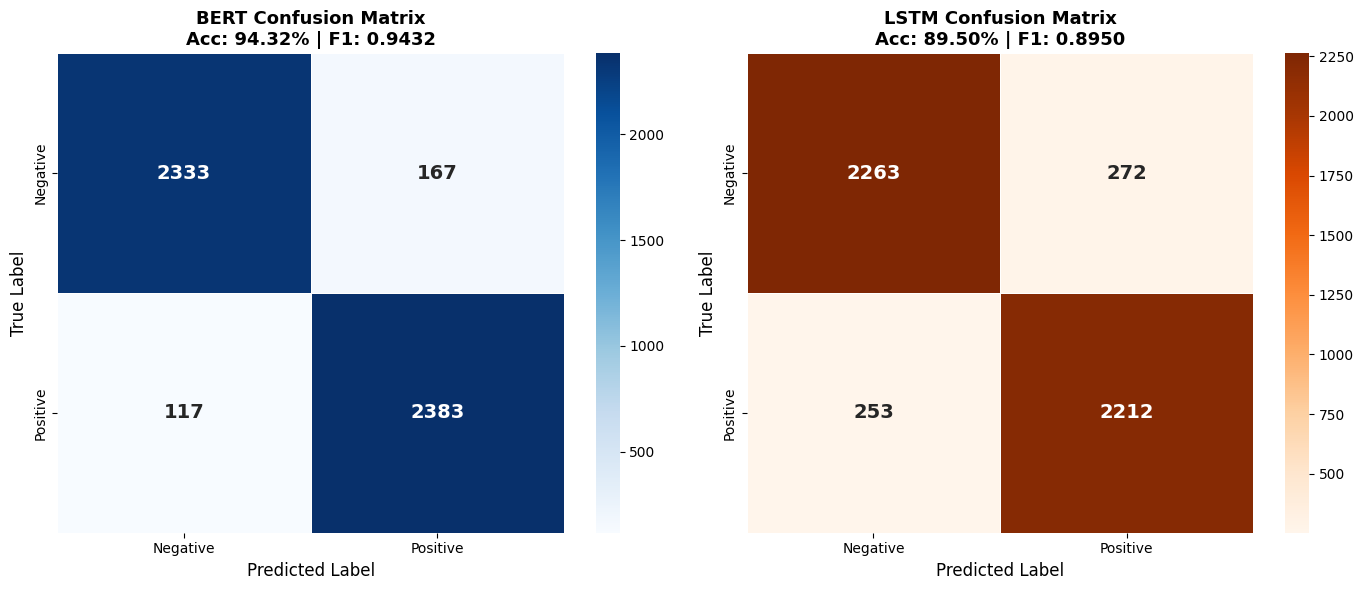
\includegraphics[width=\linewidth]{Images/text-confusionmatrix.png}
	\vspace{10pt}
	\caption{Ma trận nhầm lẫn (Confusion Matrix) của hai mô hình trên tập kiểm thử}
	\label{fig:text-confusionmatrix}
\end{figure}

\begin{enumerate}
	\item \textbf{Mô hình BERT:}
	      \begin{itemize}
		      \item True Negatives ($TN$): $2,333$ mẫu.
		      \item True Positives ($TP$): $2,383$ mẫu.
		      \item False Positives ($FP$): $167$ mẫu.
		      \item False Negatives ($FN$): $117$ mẫu.
	      \end{itemize}
	      Phân phối lỗi của BERT khá cân bằng và được nén ở mức tối thiểu. Việc $FN$ ($117$) thấp hơn $FP$ ($167$) cho thấy BERT có xu hướng "nhạy" hơn một chút trong việc phát hiện cảm xúc tích cực, đôi khi dán nhãn nhầm các câu chê bai tinh vi thành khen ngợi.

	\item \textbf{Mô hình Bi-LSTM:}
	      \begin{itemize}
		      \item True Negatives ($TN$): $2,263$ mẫu.
		      \item True Positives ($TP$): $2,212$ mẫu.
		      \item False Positives ($FP$): $272$ mẫu.
		      \item False Negatives ($FN$): $253$ mẫu.
	      \end{itemize}
	      Tổng số mẫu bị phân loại sai của LSTM là $525$ mẫu, cao hơn $84.8\%$ so với tổng số lỗi của BERT ($284$ mẫu). LSTM gặp khó khăn lớn đối với các cấu trúc ngữ pháp đảo ngược hoặc châm biếm. Khi khoảng cách vật lý giữa hư từ (như "not", "never") và tính từ gốc (như "good", "masterpiece") quá xa, lớp RNN dần quên đi bối cảnh phủ định, dẫn đến các sai số $FP$ và $FN$ gia tăng mạnh. Cơ chế Self-Attention của BERT đã khắc phục triệt để nhược điểm này bằng cách tính toán trọng số tương quan trực tiếp giữa mọi cặp từ bất chấp khoảng cách.
\end{enumerate}

\subsubsection{Đánh giá Định tính: Thử nghiệm Suy diễn (Inference Case Studies)}
Để kiểm chứng năng lực ngữ nghĩa thực tế, 5 mẫu văn bản giả định mang các sắc thái cực đoan và hỗn hợp được đưa vào hệ thống suy diễn (inference pipeline) để quan sát sự tự tin (confidence scores) của hai mô hình.

\begin{itemize}
	\item \textbf{Ca kiểm thử số 1 (Tích cực mạnh):} \textit{"An absolute masterpiece. The cinematography is stunning..."} Cả hai mô hình đều trích xuất thành công các tính từ mạnh ("masterpiece", "stunning"). BERT tự tin dự đoán POSITIVE với $99.9\%$, LSTM tự tin tuyệt đối $100.0\%$.
	\item \textbf{Ca kiểm thử số 2 (Tiêu cực mạnh):} \textit{"What a complete waste of time and money..."} Các ngữ nghĩa "waste", "wooden" giúp hai mô hình dễ dàng dán nhãn NEGATIVE với sự tự tin cực đại (BERT $99.9\%$, LSTM $100.0\%$).
	\item \textbf{Ca kiểm thử số 3 (Cảm xúc hỗn hợp/Phân cực chìm):} \textit{"It was okay, nothing special. Some scenes were interesting but the pacing felt off. Probably wouldn't watch it again."} \\
	      Đây là một mẫu văn bản bẫy thuật toán (adversarial example) khi đan xen các từ có vẻ tích cực ("okay", "interesting") bên trong một đánh giá tiêu cực tổng thể.
	      \begin{itemize}
		      \item Mô hình BERT xử lý xuất sắc, triệt tiêu nhiễu từ các từ tích cực và dán nhãn NEGATIVE với xác suất $99.8\%$.
		      \item Mô hình Bi-LSTM, do bị tác động bởi các hàm lượng thông tin tích cực xuất hiện rải rác, đã bị giảm độ tự tin xuống còn $97.8\%$, phân bổ $2.2\%$ xác suất cho lớp POSITIVE. Sự dao động này phản ánh hạn chế trong việc tổng hợp ngữ nghĩa toàn cục của mạng quy hồi.
	      \end{itemize}
	\item \textbf{Ca kiểm thử số 4 và 5:} Cả hai mô hình tiếp tục thể hiện sự ổn định khi nhận diện chính xác câu khen ngợi đạo diễn Nolan (POSITIVE) và câu chê bai CGI tệ hại (NEGATIVE) với độ tin cậy gần như tuyệt đối.
\end{itemize}

\subsubsection{Tiểu kết}
Kết quả thực nghiệm đã minh chứng định lượng sức mạnh biểu diễn vượt trội của mô hình BERT. Bằng cách tận dụng cơ chế Tự chú ý và không gian kiến thức học chuyển giao, BERT không chỉ thiết lập mức hiệu suất $94.32\%$ mà còn duy trì độ bền vững tuyệt đối trước các văn bản có cấu trúc đánh lừa. Về phần mình, kiến trúc Bi-LSTM với ma trận GloVe, dù có hiện tượng quá khớp và độ chính xác thấp hơn ($89.50\%$), vẫn chứng minh được giá trị thực tiễn trong các bài toán yêu cầu chi phí tham số thấp và tốc độ suy diễn nhanh.

%%%%%%%%%%%%%%%%%%%%%%%%%%%%%%%%%
% PHẦN MỚI: Phân loại Đa phương thức với CLIP
%%%%%%%%%%%%%%%%%%%%%%%%%%%%%%%%%
\section{Phân loại Đa phương thức với CLIP}\label{sec:multimodal}

\subsection{Giới thiệu}
Phân loại đa phương thức (Multimodal Classification) là bài toán nhận dạng và phân loại dữ liệu từ nhiều nguồn thông tin khác nhau, trong đó phổ biến nhất là sự kết hợp giữa \textbf{hình ảnh} và \textbf{văn bản}. Khác với phân loại đơn phương thức truyền thống (chỉ dùng ảnh hoặc chỉ dùng text), phương pháp đa phương thức có khả năng tận dụng thông tin bổ sung từ nhiều modality để cải thiện độ chính xác.

Trong phần này, chúng tôi thực hiện so sánh \textbf{ba phương pháp} phân loại đa phương thức trên tập dữ liệu COCO (Common Objects in Context), sử dụng mô hình CLIP (Contrastive Language-Image Pre-training) từ OpenAI:

\begin{enumerate}
    \item \textbf{Zero-shot Classification}: Phân loại trực tiếp mà không cần huấn luyện thêm.
    \item \textbf{Few-shot Classification (Frozen Backbone)}: Tinh chỉnh đầu phân loại với số lượng mẫu nhỏ (k=1,5,10,20), giữ nguyên trọng số của mạng nền CLIP.
    \item \textbf{Full Fine-Tuning (Unfrozen Backbone)}: Tinh chỉnh toàn bộ mô hình CLIP với lượng dữ liệu lớn hơn (100 samples/class).
\end{enumerate}

\subsection{Tập dữ liệu COCO 2017}\label{subsec:coco-dataset}

\subsubsection{Giới thiệu về COCO}
COCO (Common Objects in Context) là một trong những tập dữ liệu chuẩn quốc tế quan trọng nhất cho các bài toán thị giác máy tính, bao gồm:
\begin{itemize}
    \item \textbf{Object Detection} (Phát hiện đối tượng)
    \item \textbf{Instance Segmentation} (Phân đoạn thực thể)
    \item \textbf{Image Captioning} (Mô tả ảnh)
    \item \textbf{Multimodal Classification} (Phân loại đa phương thức)
\end{itemize}

Tập dữ liệu gốc chứa \textbf{80 categories} phổ biến trong đời sống hàng ngày, từ con người, phương tiện, động vật đến đồ vật gia dụng. Mỗi ảnh trong COCO đi kèm với:
\begin{itemize}
    \item \textbf{Annotations}: Bounding boxes, segmentation masks
    \item \textbf{Captions}: 5 câu mô tả tiếng Anh cho mỗi ảnh
    \item \textbf{Category labels}: Nhãn phân loại đối tượng
\end{itemize}

\subsubsection{Xử lý và Lọc Dữ liệu}
Trong thực nghiệm này, chúng tôi sử dụng phiên bản COCO 2017 từ Kaggle\footnote{Kaggle COCO Dataset: \url{https://www.kaggle.com/datasets/awsaf49/coco-2017-dataset}}. Quy trình xử lý dữ liệu bao gồm:

\begin{enumerate}
    \item \textbf{Kết hợp train và validation splits}: Gộp cả train2017 và val2017 để tăng số lượng mẫu.
    \item \textbf{Lọc categories thiếu dữ liệu}: Loại bỏ các categories có ít hơn 100 samples để đảm bảo chất lượng huấn luyện.
    \item \textbf{Primary category assignment}: Với mỗi ảnh chứa nhiều đối tượng, chọn đối tượng có diện tích lớn nhất làm category chính.
    \item \textbf{Caption extraction}: Lấy caption đầu tiên cho mỗi ảnh làm thông tin văn bản.
\end{enumerate}

Sau khi xử lý, tập dữ liệu cuối cùng có các thông số sau:

\begin{table}[H]
    \centering
    \caption{Thống kê tập dữ liệu COCO sau xử lý}
    \begin{tabular}{|l|r|}
        \hline
        \textbf{Thuộc tính} & \textbf{Giá trị} \\
        \hline
        Tổng số categories & 43 \\
        \hline
        Tổng số samples & 4,424 \\
        \hline
        Samples per class & 100-103 \\
        \hline
        Training set (80\%) & 3,539 \\
        \hline
        Test set (20\%) & 885 \\
        \hline
        Modality & Image + Text (caption) \\
        \hline
    \end{tabular}
    \label{tab:coco-stats}
\end{table}

\textbf{43 categories} được giữ lại bao gồm: person, dog, bowl, bench, toilet, motorcycle, boat, bed, giraffe, car, zebra, chair, airplane, umbrella, bus, cow, dining table, teddy bear, couch, horse, bird, elephant, sheep, clock, train, bicycle, truck, oven, refrigerator, pizza, stop sign, kite, sink, sandwich, cat, fire hydrant, tv, traffic light, bear, suitcase, laptop, surfboard, vase.

\subsection{Kiến trúc CLIP}\label{subsec:clip-architecture}

\subsubsection{Tổng quan về CLIP}
CLIP (Contrastive Language-Image Pre-training) là mô hình đột phá từ OpenAI, được giới thiệu năm 2021\cite{radford2021learning}. Điểm đặc biệt của CLIP là khả năng học biểu diễn chung (joint representation) cho cả hình ảnh và văn bản thông qua huấn luyện contrastive trên \textbf{400 triệu cặp image-text} từ internet.

\begin{figure}[H]
    \centering
    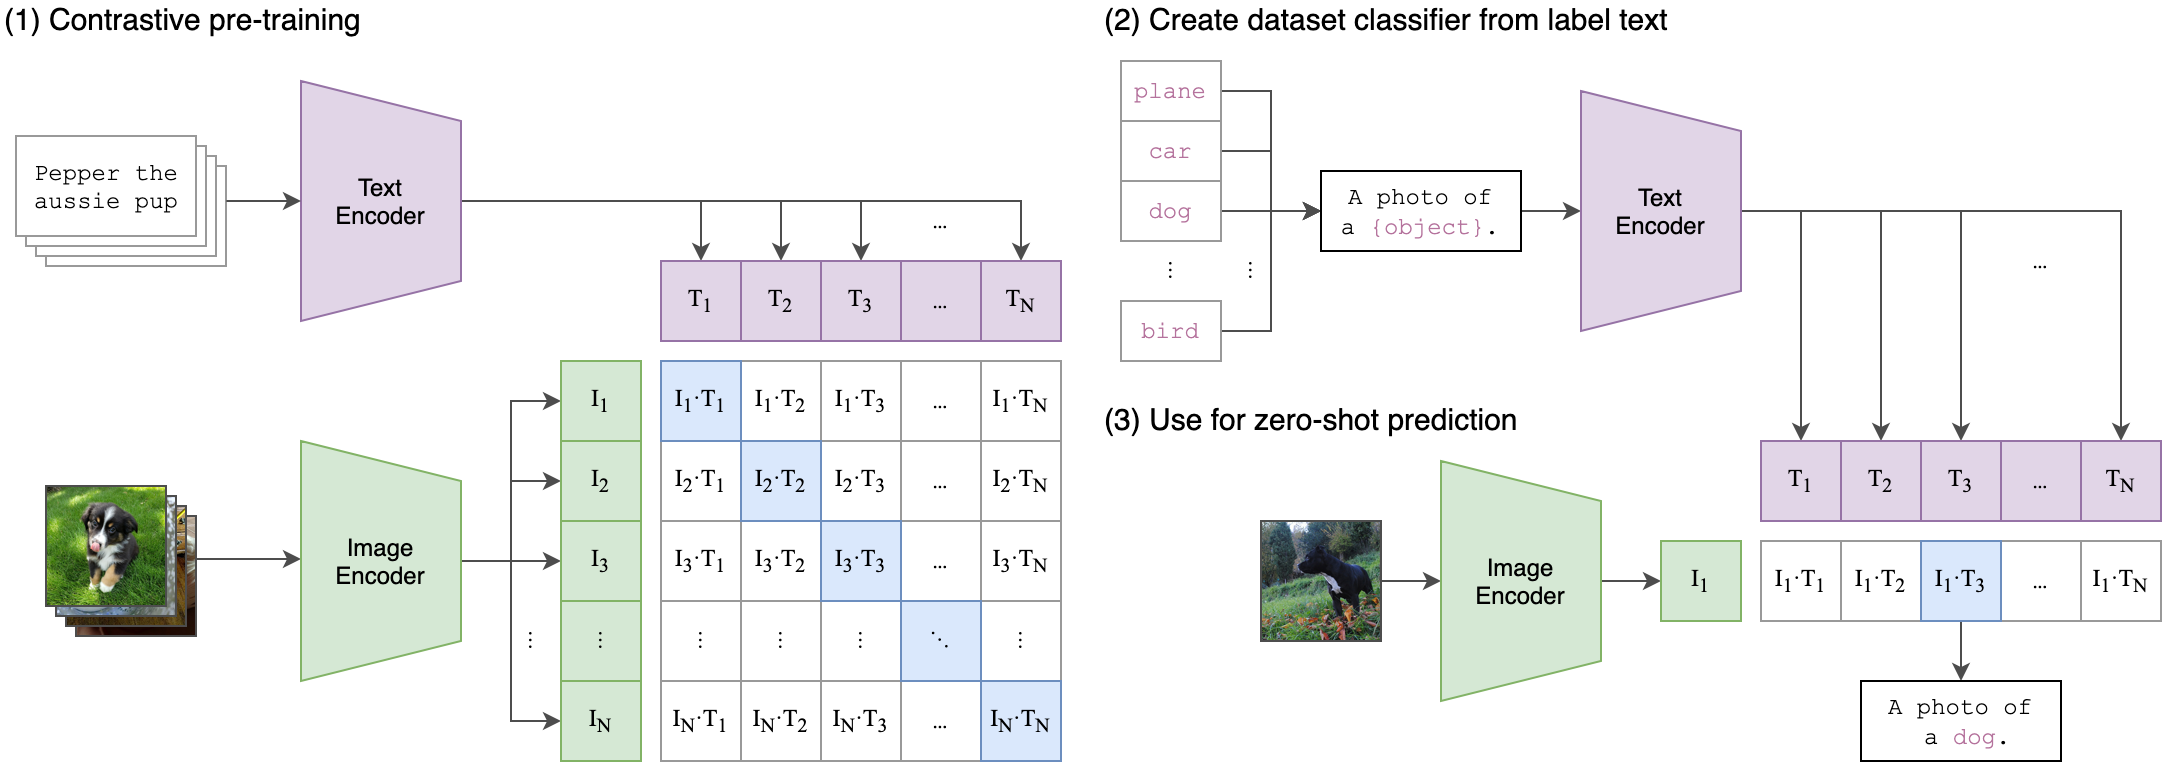
\includegraphics[width=0.95\textwidth]{Images/clip_architecture.png}

    \vspace{0.5cm}
    \caption{Kiến trúc CLIP: Vision Encoder và Text Encoder được huấn luyện để tạo ra biểu diễn tương đồng cho các cặp ảnh-văn bản phù hợp\protect\footnotemark}
    \label{fig:clip-architecture}
\end{figure}
\footnotetext{Nguồn: OpenAI CLIP repository - \url{https://github.com/openai/CLIP}}

\subsubsection{Các thành phần chính}
CLIP bao gồm hai encoder hoạt động song song:

\paragraph{Vision Encoder}
Sử dụng kiến trúc \textbf{Vision Transformer (ViT)} với patch size 32x32. Mô hình chia ảnh đầu vào thành các patches nhỏ, sau đó xử lý chúng như một chuỗi tokens tương tự như trong NLP.

\begin{itemize}
    \item \textbf{Input}: Ảnh RGB kích thước $224 \times 224$ pixels
    \item \textbf{Patch embedding}: Chia thành $7 \times 7 = 49$ patches
    \item \textbf{Transformer layers}: 12 layers với multi-head attention
    \item \textbf{Output}: Image embedding vector $\in \mathbb{R}^{512}$
\end{itemize}

\paragraph{Text Encoder}
Sử dụng kiến trúc \textbf{Transformer} để mã hóa câu văn bản thành vector đặc trưng.

\begin{itemize}
    \item \textbf{Input}: Text sequence (max 77 tokens)
    \item \textbf{Tokenization}: Byte-Pair Encoding (BPE)
    \item \textbf{Transformer layers}: 12 layers với causal attention
    \item \textbf{Output}: Text embedding vector $\in \mathbb{R}^{512}$
\end{itemize}

\subsubsection{Contrastive Learning}
CLIP được huấn luyện với mục tiêu contrastive: tối đa hóa cosine similarity giữa các cặp (image, text) đúng và tối thiểu hóa similarity giữa các cặp không khớp. Hàm loss được định nghĩa:

\begin{equation}
    \mathcal{L}_{\text{CLIP}} = \frac{1}{2}\left(\mathcal{L}_{\text{I2T}} + \mathcal{L}_{\text{T2I}}\right)
\end{equation}

Trong đó:
\begin{itemize}
    \item $\mathcal{L}_{\text{I2T}}$: Cross-entropy loss từ image sang text
    \item $\mathcal{L}_{\text{T2I}}$: Cross-entropy loss từ text sang image
\end{itemize}

\subsubsection{Tại sao CLIP phù hợp cho Multimodal Classification?}
\begin{enumerate}
    \item \textbf{Pre-trained trên dữ liệu đa dạng}: 400M cặp image-text từ internet.
    \item \textbf{Zero-shot capability}: Có thể phân loại các class chưa từng thấy trong quá trình huấn luyện.
    \item \textbf{Joint embedding space}: Biểu diễn ảnh và text trong cùng một không gian vector.
    \item \textbf{Transfer learning friendly}: Dễ dàng fine-tune cho các tác vụ downstream.
\end{enumerate}

\subsection{Ba Phương pháp So sánh}\label{subsec:three-methods}

\subsubsection{Zero-Shot Classification}\label{subsubsec:zero-shot}

\paragraph{Khái niệm}
Zero-shot classification là phương pháp phân loại \textbf{không cần huấn luyện thêm} (no additional training). Mô hình CLIP pretrained được sử dụng trực tiếp để phân loại các ảnh bằng cách so sánh chúng với các text prompts tương ứng với mỗi category.

\paragraph{Cơ chế hoạt động}
\begin{enumerate}
    \item \textbf{Tạo text prompts}: Với mỗi category $c$, tạo prompt theo template: \texttt{"a photo of a \{category\}"}

    Ví dụ:
    \begin{itemize}
        \item Category "person" → \texttt{"a photo of a person"}
        \item Category "car" → \texttt{"a photo of a car"}
    \end{itemize}

    \item \textbf{Encode image và text}:
    \begin{align}
        \mathbf{v}_{\text{img}} &= \text{VisionEncoder}(\text{image}) \\
        \mathbf{v}_{\text{text}}^{(i)} &= \text{TextEncoder}(\text{prompt}_i), \quad i=1,\ldots,C
    \end{align}

    \item \textbf{Tính similarity scores}:
    \begin{equation}
        s_i = \cos(\mathbf{v}_{\text{img}}, \mathbf{v}_{\text{text}}^{(i)}) = \frac{\mathbf{v}_{\text{img}} \cdot \mathbf{v}_{\text{text}}^{(i)}}{\|\mathbf{v}_{\text{img}}\| \|\mathbf{v}_{\text{text}}^{(i)}\|}
    \end{equation}

    \item \textbf{Dự đoán category}:
    \begin{equation}
        \hat{y} = \arg\max_{i} \, \text{softmax}(s_i / \tau)
    \end{equation}

    Trong đó $\tau$ là temperature parameter (thường = 0.01).
\end{enumerate}

\paragraph{Ưu điểm}
\begin{itemize}
    \item Không cần dữ liệu huấn luyện
    \item Thời gian inference nhanh (không có training phase)
    \item Có thể mở rộng sang các class mới ngay lập tức
    \item Tận dụng tối đa knowledge từ pretrained model
\end{itemize}

\paragraph{Nhược điểm}
\begin{itemize}
    \item Không customize được cho dataset cụ thể
    \item Performance bị giới hạn bởi pretrained knowledge
    \item Có thể kém hiệu quả với domain-specific tasks
\end{itemize}

\paragraph{Cấu hình thực nghiệm}
\begin{table}[H]
    \centering
    \caption{Thông số Zero-shot Classification}
    \begin{tabular}{|l|l|}
        \hline
        \textbf{Tham số} & \textbf{Giá trị} \\
        \hline
        Model & openai/clip-vit-base-patch32 \\
        \hline
        Training data & 0 samples \\
        \hline
        Trainable parameters & 0 (all frozen) \\
        \hline
        Training time & 0s \\
        \hline
        Prompt template & "a photo of a \{category\}" \\
        \hline
        Temperature $\tau$ & 0.01 \\
        \hline
    \end{tabular}
    \label{tab:zero-shot-config}
\end{table}

\subsubsection{Few-Shot Classification (Frozen Backbone)}\label{subsubsec:few-shot}

\paragraph{Khái niệm}
Few-shot classification là phương pháp huấn luyện mô hình với \textbf{số lượng mẫu rất nhỏ} cho mỗi class (thường từ 1-20 samples). Trong phương pháp này, backbone CLIP được \textbf{đóng băng} (frozen), chỉ có classification head được huấn luyện.

\paragraph{Kiến trúc}
Mô hình bao gồm hai phần chính:

\begin{enumerate}
    \item \textbf{CLIP Encoder (FROZEN)}:
    \begin{itemize}
        \item Vision Encoder: xử lý ảnh → image embedding
        \item Text Encoder: xử lý caption → text embedding
        \item Tất cả trọng số của CLIP đều \texttt{requires\_grad=False}
    \end{itemize}

    \item \textbf{Classification Head (TRAINABLE)}:
    \begin{itemize}
        \item Input: Concatenation của image embedding và text embedding
        \item Architecture: 2-layer MLP
        \item Layer 1: Linear($512 \times 2 = 1024$, 512) + ReLU + Dropout(0.1)
        \item Layer 2: Linear(512, num\_classes)
        \item Output: Logits cho 43 categories
    \end{itemize}
\end{enumerate}

\begin{minted}[linenos, breaklines, fontsize=\small]{python}
class CLIPClassifier(nn.Module):
    def __init__(self, clip_model, num_classes, freeze_backbone=True):
        super().__init__()
        self.clip = clip_model

        # Đóng băng CLIP backbone
        if freeze_backbone:
            for param in self.clip.parameters():
                param.requires_grad = False

        # Classification head (trainable)
        hidden_size = self.clip.config.projection_dim  # 512
        self.classifier = nn.Sequential(
            nn.Linear(hidden_size * 2, hidden_size),
            nn.ReLU(),
            nn.Dropout(0.1),
            nn.Linear(hidden_size, num_classes)
        )

    def forward(self, input_ids, attention_mask, pixel_values):
        outputs = self.clip(input_ids, attention_mask, pixel_values)
        combined = torch.cat([outputs.image_embeds,
                             outputs.text_embeds], dim=1)
        return self.classifier(combined)
\end{minted}

\paragraph{Cấu hình huấn luyện}
Chúng tôi thực nghiệm với \textbf{4 giá trị k khác nhau}: k=1, 5, 10, 20 samples per class.

\begin{table}[H]
    \centering
    \caption{Thông số Few-shot Classification}
    \begin{tabular}{|l|l|l|l|l|}
        \hline
        \textbf{Tham số} & \textbf{1-shot} & \textbf{5-shot} & \textbf{10-shot} & \textbf{20-shot} \\
        \hline
        Training samples & 43 & 215 & 430 & 860 \\
        \hline
        Samples/class & 1 & 5 & 10 & 20 \\
        \hline
        Epochs & 20 & 20 & 10 & 10 \\
        \hline
        Learning rate & 1e-4 & 1e-4 & 5e-5 & 5e-5 \\
        \hline
        Batch size & 8 & 8 & 8 & 8 \\
        \hline
        Optimizer & \multicolumn{4}{c|}{AdamW} \\
        \hline
        Trainable params & \multicolumn{4}{c|}{~262K (chỉ classification head)} \\
        \hline
        Frozen params & \multicolumn{4}{c|}{~151M (CLIP backbone)} \\
        \hline
    \end{tabular}
    \label{tab:few-shot-config}
\end{table}

\paragraph{Ưu điểm}
\begin{itemize}
    \item Cải thiện performance với rất ít dữ liệu
    \item Training nhanh (chỉ train head, không train backbone)
    \item Tránh overfitting nhờ freeze pretrained weights
    \item Giữ lại được generalization capability của CLIP
\end{itemize}

\paragraph{Nhược điểm}
\begin{itemize}
    \item Performance bị giới hạn bởi frozen features
    \item Không thể adapt backbone cho domain-specific patterns
    \item Với k quá nhỏ (k=1), performance vẫn rất thấp
\end{itemize}

\subsubsection{Full Fine-Tuning (Unfrozen Backbone)}\label{subsubsec:full-finetune}

\paragraph{Khái niệm}
Full fine-tuning là phương pháp huấn luyện \textbf{toàn bộ mô hình}, bao gồm cả CLIP backbone. Khác với few-shot learning, ở đây tất cả các layers đều có thể cập nhật trọng số (\texttt{requires\_grad=True}).

\paragraph{Điểm khác biệt chính}
\begin{table}[H]
    \centering
    \caption{So sánh Few-shot (Frozen) vs Full Fine-tuning (Unfrozen)}
    \begin{tabular}{|l|l|l|}
        \hline
        \textbf{Aspect} & \textbf{Few-shot (Frozen)} & \textbf{Full Fine-tune (Unfrozen)} \\
        \hline
        Backbone status & \texttt{freeze\_backbone=True} & \texttt{freeze\_backbone=False} \\
        \hline
        Trainable layers & Chỉ classification head & Toàn bộ model \\
        \hline
        Trainable params & ~262K & ~546K \\
        \hline
        Training data & 1-20 samples/class & 100 samples/class \\
        \hline
        Learning rate & 1e-4 hoặc 5e-5 & 2e-5 (thấp hơn) \\
        \hline
        Epochs & 10-20 & 5 (ít hơn) \\
        \hline
        Risk of overfitting & Thấp & Cao hơn \\
        \hline
        Training time & Nhanh (~85-137s) & Chậm hơn (~151s) \\
        \hline
    \end{tabular}
    \label{tab:frozen-vs-unfrozen}
\end{table}

\paragraph{Cấu hình huấn luyện}
\begin{table}[H]
    \centering
    \caption{Thông số Full Fine-Tuning}
    \begin{tabular}{|l|l|}
        \hline
        \textbf{Tham số} & \textbf{Giá trị} \\
        \hline
        Training samples & 3,539 (100 samples/class) \\
        \hline
        Epochs & 5 \\
        \hline
        Learning rate & 2e-5 (thấp để stability) \\
        \hline
        Batch size & 8 \\
        \hline
        Optimizer & AdamW \\
        \hline
        Scheduler & Linear warmup (10\% steps) \\
        \hline
        Trainable params & ~546K (toàn bộ model) \\
        \hline
        freeze\_backbone & False \\
        \hline
    \end{tabular}
    \label{tab:full-finetune-config}
\end{table}

\paragraph{Ưu điểm}
\begin{itemize}
    \item Tiềm năng đạt accuracy cao nhất
    \item Có thể adapt toàn bộ model cho domain-specific task
    \item Học được patterns phức tạp hơn từ dữ liệu
\end{itemize}

\paragraph{Nhược điểm}
\begin{itemize}
    \item Cần nhiều dữ liệu hơn (ít nhất 50-100 samples/class)
    \item Training chậm hơn (train toàn bộ 151M parameters)
    \item Nguy cơ overfitting cao nếu dữ liệu không đủ
    \item Có thể mất đi generalization capability của pretrained model
\end{itemize}

\subsection{Thiết lập Thực nghiệm}\label{subsec:experiment-setup}

\subsubsection{Môi trường và Phần cứng}
\begin{itemize}
    \item \textbf{Platform}: Kaggle Notebook
    \item \textbf{GPU}: Tesla T4 x2 (16GB VRAM mỗi card)
    \item \textbf{Framework}: PyTorch 2.x, Transformers (HuggingFace)
    \item \textbf{Python}: 3.10
\end{itemize}

\subsubsection{Chia tách dữ liệu}
\begin{itemize}
    \item \textbf{Test set}: 20\% (885 samples) - stratified by category
    \item \textbf{Training set}: 80\% (3,539 samples)
    \begin{itemize}
        \item Few-shot: Lấy ngẫu nhiên k samples/class (k=1,5,10,20)
        \item Full fine-tune: Sử dụng toàn bộ 100 samples/class
    \end{itemize}
\end{itemize}

\subsubsection{Metrics đánh giá}
Theo yêu cầu của đề bài (Section 4.4), chúng tôi đánh giá tất cả các phương pháp với các metrics sau:

\begin{enumerate}
    \item \textbf{Accuracy}: Tỷ lệ phân loại đúng tổng thể
    \begin{equation}
        \text{Accuracy} = \frac{\text{Số lượng dự đoán đúng}}{\text{Tổng số mẫu}}
    \end{equation}

    \item \textbf{F1 Score (Macro)}: Trung bình cộng F1 của từng class
    \begin{equation}
        F1_{\text{macro}} = \frac{1}{C}\sum_{i=1}^{C} F1_i
    \end{equation}

    \item \textbf{F1 Score (Weighted)}: Trung bình có trọng số theo số lượng samples
    \begin{equation}
        F1_{\text{weighted}} = \sum_{i=1}^{C} w_i \cdot F1_i, \quad w_i = \frac{n_i}{\sum_j n_j}
    \end{equation}

    \item \textbf{Precision (Macro)}: Độ chính xác trung bình
    \item \textbf{Recall (Macro)}: Độ phủ trung bình
    \item \textbf{Confusion Matrix}: Ma trận nhầm lẫn 43x43
    \item \textbf{Per-class Metrics}: F1, Precision, Recall cho từng category
\end{enumerate}

\subsection{Kết quả và Phân tích}\label{subsec:results}

\subsubsection{So sánh Tổng quan}
Bảng~\ref{tab:overall-comparison} tổng hợp kết quả của tất cả 6 thí nghiệm (1 zero-shot + 4 few-shot + 1 full fine-tuning).

\begin{table}[H]
    \centering
    \caption{So sánh tổng quan: Zero-shot vs Few-shot vs Full Fine-tuning}
    \begin{tabular}{|l|r|l|r|r|r|r|r|}
        \hline
        \textbf{Method} & \textbf{K} & \textbf{Backbone} & \textbf{Acc} & \textbf{F1 Ma} & \textbf{F1 We} & \textbf{Prec} & \textbf{Recall} \\
        \hline
        Zero-Shot & 0 & Frozen & \textbf{0.758} & \textbf{0.741} & \textbf{0.740} & 0.754 & 0.759 \\
        \hline
        1-Shot & 1 & Frozen & 0.162 & 0.106 & 0.106 & 0.189 & 0.161 \\
        \hline
        5-Shot & 5 & Frozen & 0.645 & 0.614 & 0.614 & 0.672 & 0.645 \\
        \hline
        10-Shot & 10 & Frozen & 0.399 & 0.367 & 0.367 & 0.487 & 0.398 \\
        \hline
        20-Shot & 20 & Frozen & 0.652 & 0.616 & 0.615 & 0.671 & 0.652 \\
        \hline
        Full FT & 100 & Unfrozen & 0.644 & 0.602 & 0.600 & \textbf{0.653} & \textbf{0.645} \\
        \hline
    \end{tabular}
    \label{tab:overall-comparison}
\end{table}

\textbf{Chú thích}: Acc = Accuracy, F1 Ma = F1 Macro, F1 We = F1 Weighted, Prec = Precision Macro, FT = Fine-Tuning

\paragraph{Quan sát chính}
\begin{enumerate}
    \item \textbf{Zero-shot đạt kết quả tốt nhất} với accuracy 75.8\%, vượt trội hơn tất cả các phương pháp fine-tuning. Điều này cho thấy CLIP pretrained đã học được biểu diễn rất mạnh cho COCO dataset.

    \item \textbf{1-shot performance cực kỳ thấp} (16.2\%), chứng tỏ 1 sample/class không đủ để học được pattern phân loại.

    \item \textbf{5-shot và 20-shot đạt kết quả tương đương nhau} (~64-65\%), cho thấy diminishing returns khi tăng k từ 5 lên 20.

    \item \textbf{Full fine-tuning không vượt trội} (64.4\%), thậm chí còn kém hơn zero-shot. Dưới góc độ lý thuyết, sự sụt giảm này là minh chứng rõ rệt cho hiện tượng \textbf{"Quên thảm khốc" (Catastrophic Forgetting)}. Khi mở khóa (unfreeze) toàn bộ mạng lưới chứa khoảng 150 triệu tham số và liên tục đẩy đạo hàm cập nhật từ một lượng dữ liệu tập trung quá nhỏ (chỉ 100 mẫu/lớp), mô hình đã tự phá vỡ không gian biểu diễn tổng quát mà nó từng tích lũy từ 400 triệu ảnh pre-train. Các trọng số bị "bẻ cong" (bias) thái quá về phía tập phân bố của COCO, hệ quả là mất đi khả năng tổng quát hóa ban đầu.
\end{enumerate}

\subsubsection{Thời gian Huấn luyện và Inference}
\begin{table}[H]
    \centering
    \caption{Phân tích thời gian xử lý}
    \begin{tabular}{|l|r|r|}
        \hline
        \textbf{Method} & \textbf{Training Time (s)} & \textbf{Inference Time (s)} \\
        \hline
        Zero-Shot & 0 & 23.5 \\
        \hline
        1-Shot & 108.5 & 5.2 \\
        \hline
        5-Shot & 136.6 & 5.3 \\
        \hline
        10-Shot & 85.0 & 5.3 \\
        \hline
        20-Shot & 113.9 & 5.2 \\
        \hline
        Full Fine-tuning & 150.7 & 5.2 \\
        \hline
    \end{tabular}
    \label{tab:time-analysis}
\end{table}

\textbf{Nhận xét}:
\begin{itemize}
    \item Zero-shot có inference time cao nhất (23.5s) vì phải encode 43 text prompts cho mỗi batch.
    \item Các phương pháp fine-tuning có inference nhanh hơn (~5s) vì chỉ cần forward pass qua classification head.
    \item Training time tăng dần từ few-shot (85-137s) đến full fine-tuning (151s).
\end{itemize}

\subsubsection{Phân tích theo K (Samples per Class)}
Hình~\ref{fig:metrics-vs-k} cho thấy xu hướng thay đổi của accuracy và F1 macro theo số lượng samples per class.

\begin{figure}[H]
    \centering
    \begin{subfigure}[b]{0.48\textwidth}
        \centering
        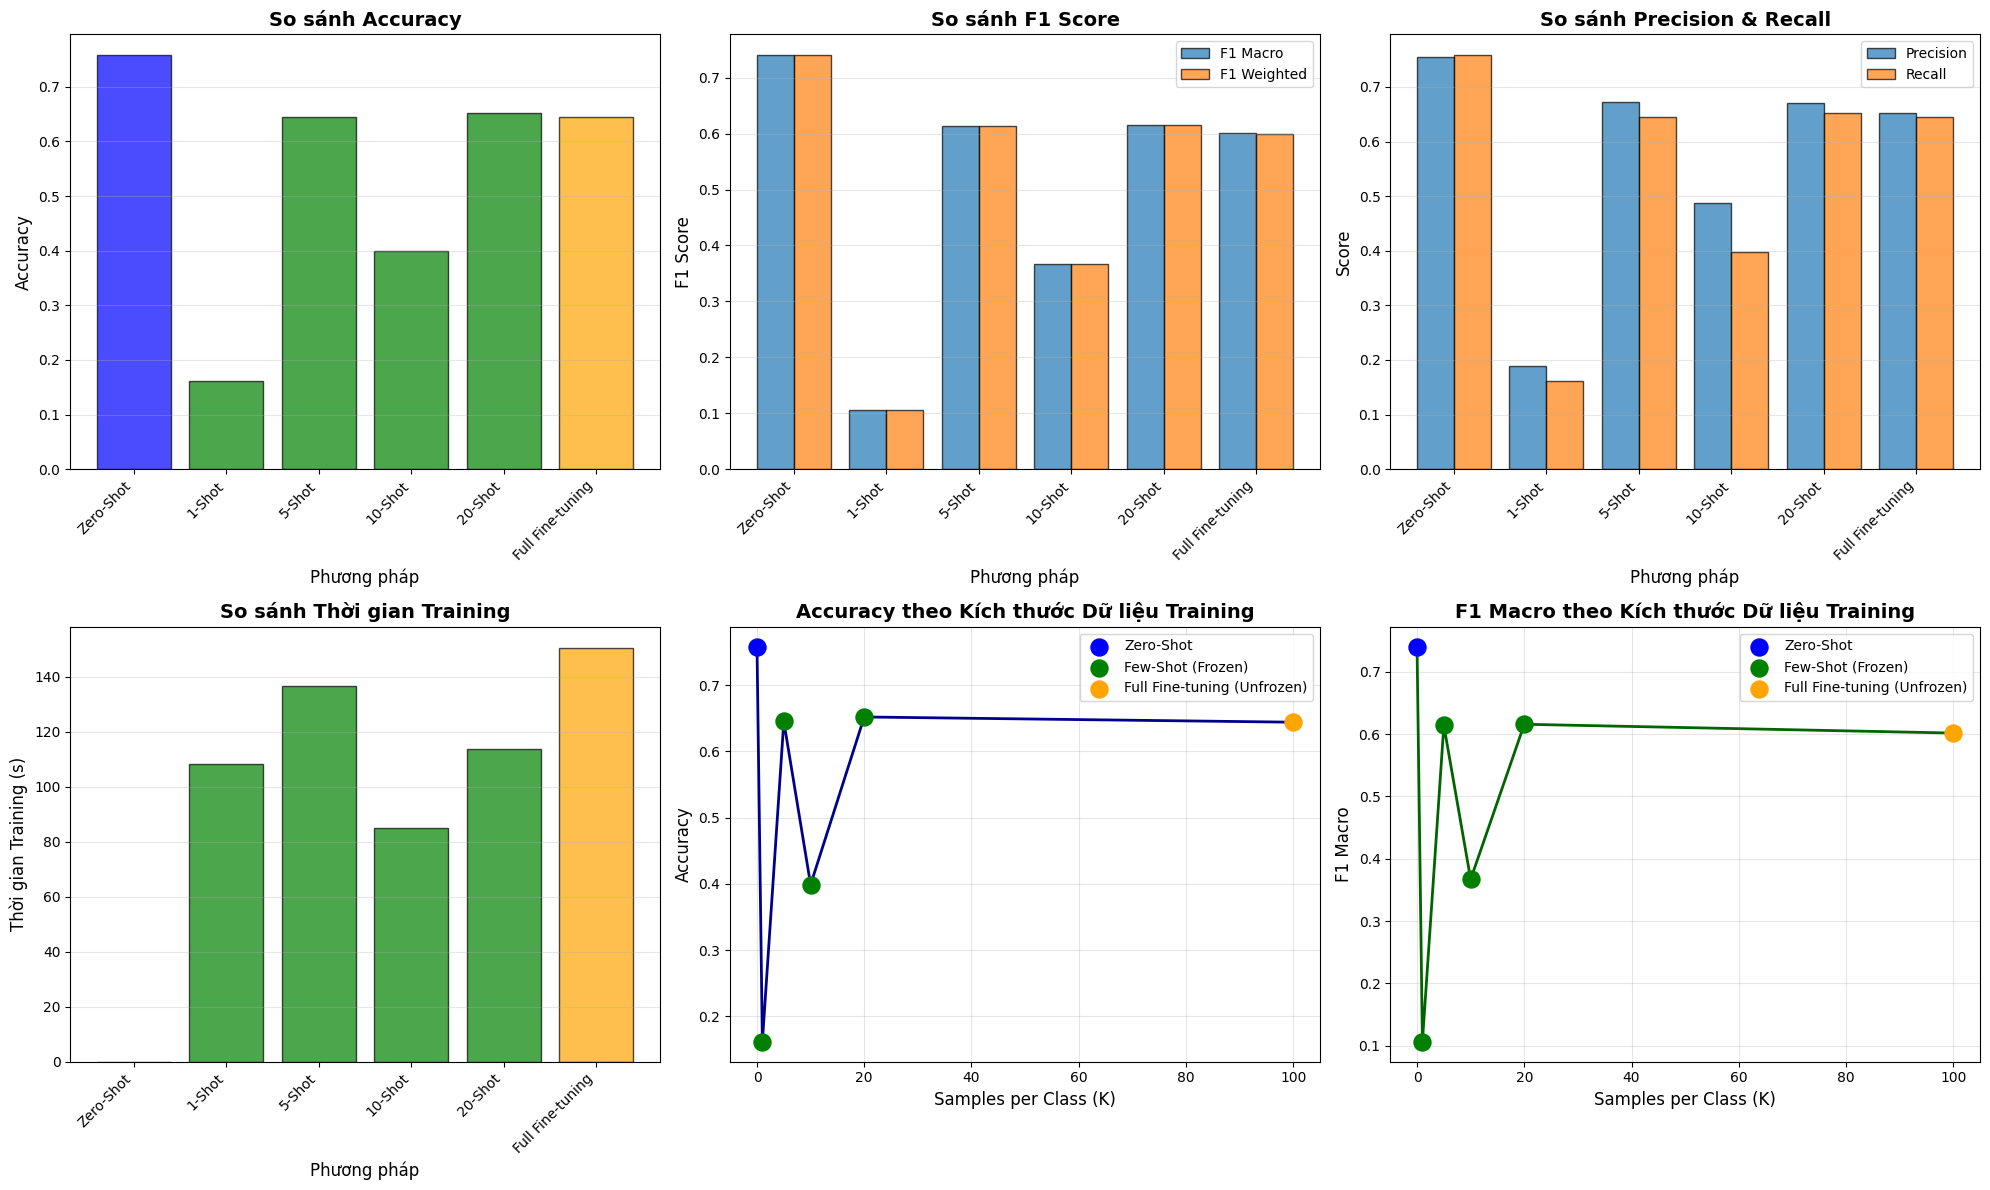
\includegraphics[width=\textwidth]{Images/multimodal_accuracy_vs_k.png}
        \caption{Accuracy theo số lượng samples per class (K)}
        \label{fig:accuracy-vs-k}
    \end{subfigure}
    \hfill
    \begin{subfigure}[b]{0.48\textwidth}
        \centering
        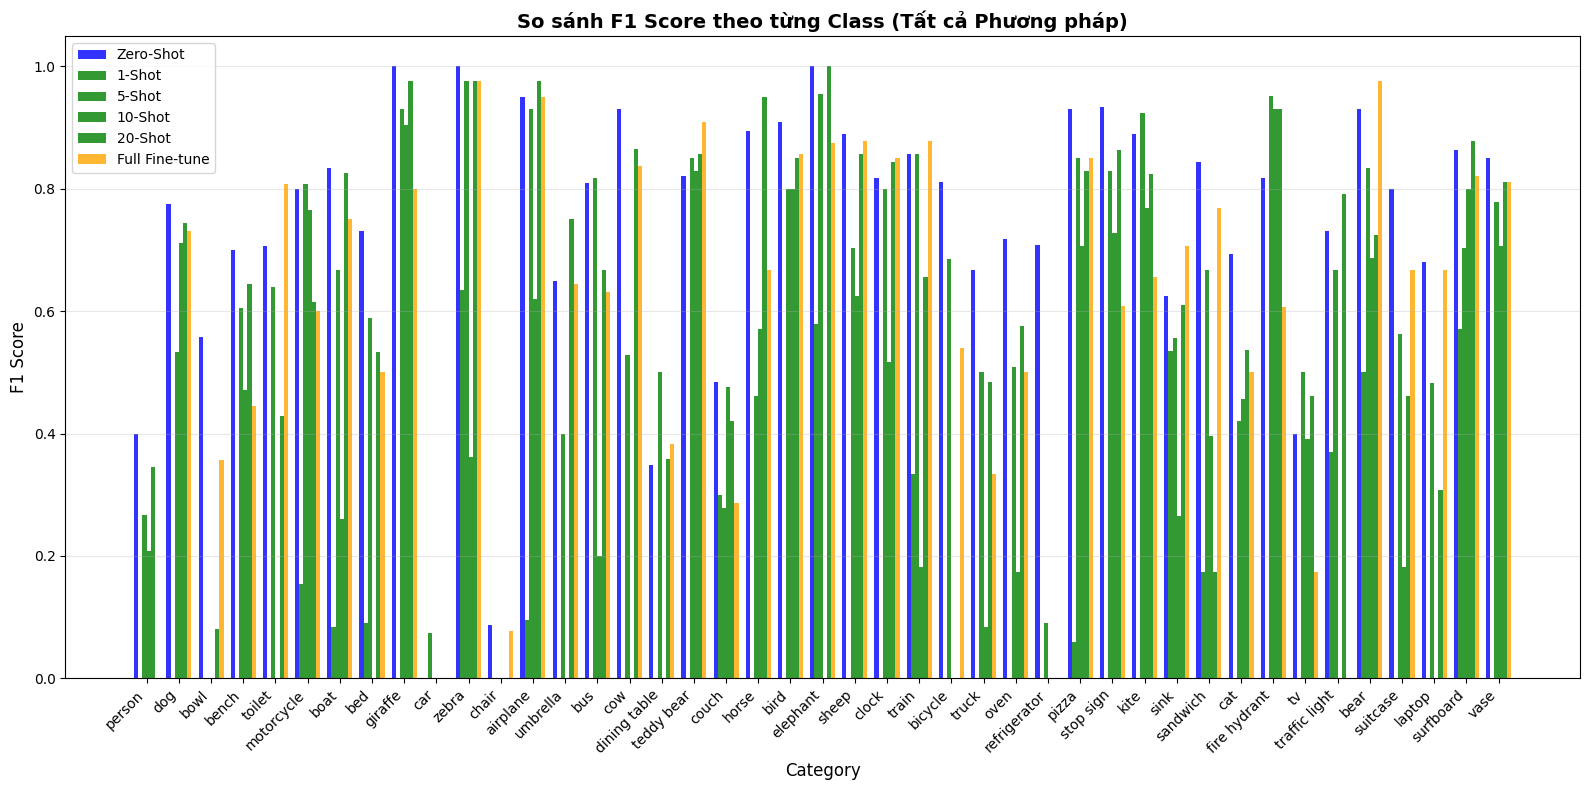
\includegraphics[width=\textwidth]{Images/multimodal_f1_vs_k.png}
        \caption{F1 Macro theo số lượng samples per class (K)}
        \label{fig:f1-vs-k}
    \end{subfigure}

    \vspace{0.5cm}
    \caption{Xu hướng thay đổi metrics theo K. Quan sát: performance tăng mạnh từ k=1 đến k=5, sau đó có diminishing returns.}
    \label{fig:metrics-vs-k}
\end{figure}

\textbf{Quan sát}:
\begin{itemize}
    \item Accuracy tăng mạnh từ k=1 (16\%) lên k=5 (64.5\%)
    \item Từ k=5 trở đi, accuracy gần như không tăng (k=5: 64.5\%, k=20: 65.2\%)
    \item Full fine-tuning (k=100) cũng chỉ đạt 64.4\%, tương đương k=5
    \item Điều này chứng tỏ: \textbf{k=5 đã đủ để đạt performance tốt} với frozen backbone
\end{itemize}

\subsubsection{Confusion Matrices}
Hình~\ref{fig:confusion-matrices} trình bày confusion matrices cho ba phương pháp đại diện: Zero-shot, 5-shot (frozen), và Full fine-tuning (unfrozen).

\begin{figure}[H]
    \centering
    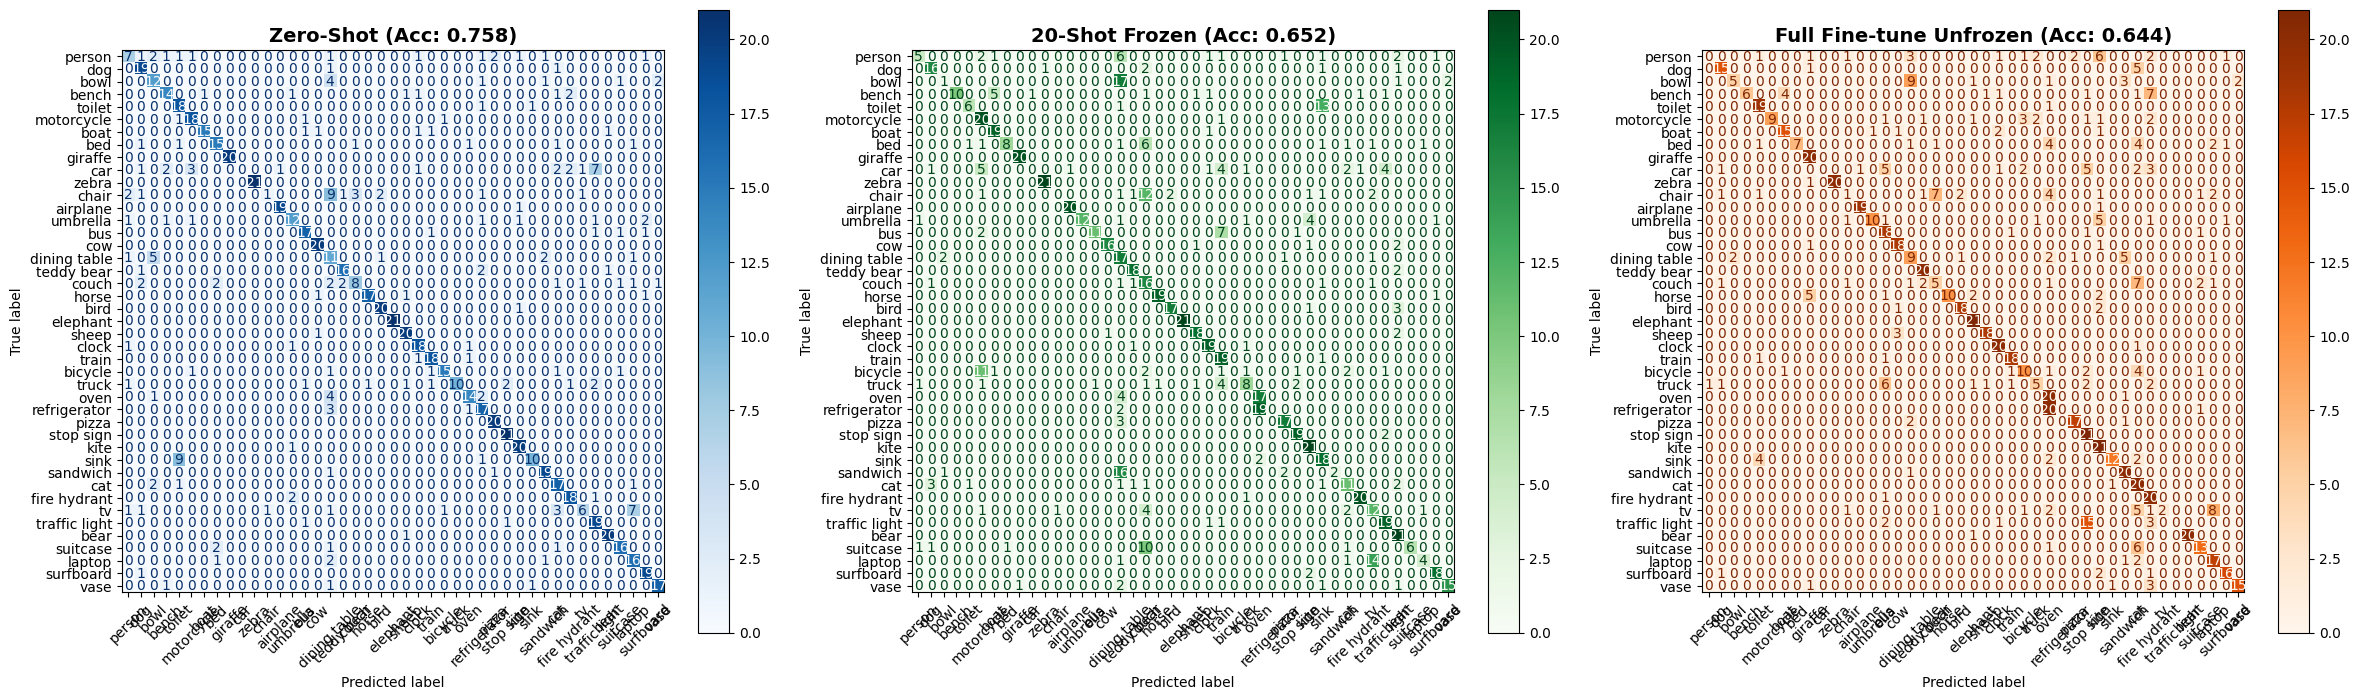
\includegraphics[width=0.95\textwidth]{Images/multimodal_cm_all_three.png}

    \vspace{0.5cm}
    \caption{Confusion matrices cho ba phương pháp (Zero-shot: 75.8\%, 5-Shot: 64.5\%, Full Fine-tune: 64.4\%). Zero-shot có đường chéo chính rõ nhất, cho thấy ít confusion giữa các classes.}
    \label{fig:confusion-matrices}
\end{figure}

\textbf{Phân tích}:
\begin{itemize}
    \item \textbf{Zero-shot}: Đường chéo chính rất nổi bật, ít confusion giữa các classes. Cho thấy CLIP pretrained phân biệt tốt các categories COCO.

    \item \textbf{5-shot}: Có một số confusion tăng lên so với zero-shot, đặc biệt ở các classes tương tự nhau (ví dụ: chair vs couch, car vs truck).

    \item \textbf{Full fine-tuning}: Tương tự 5-shot, không cải thiện đáng kể về confusion patterns.
\end{itemize}

\subsubsection{Per-class Performance}
Phân tích chi tiết F1 score của từng category (Hình~\ref{fig:per-class-f1}) cho thấy:

\begin{figure}[H]
    \centering
    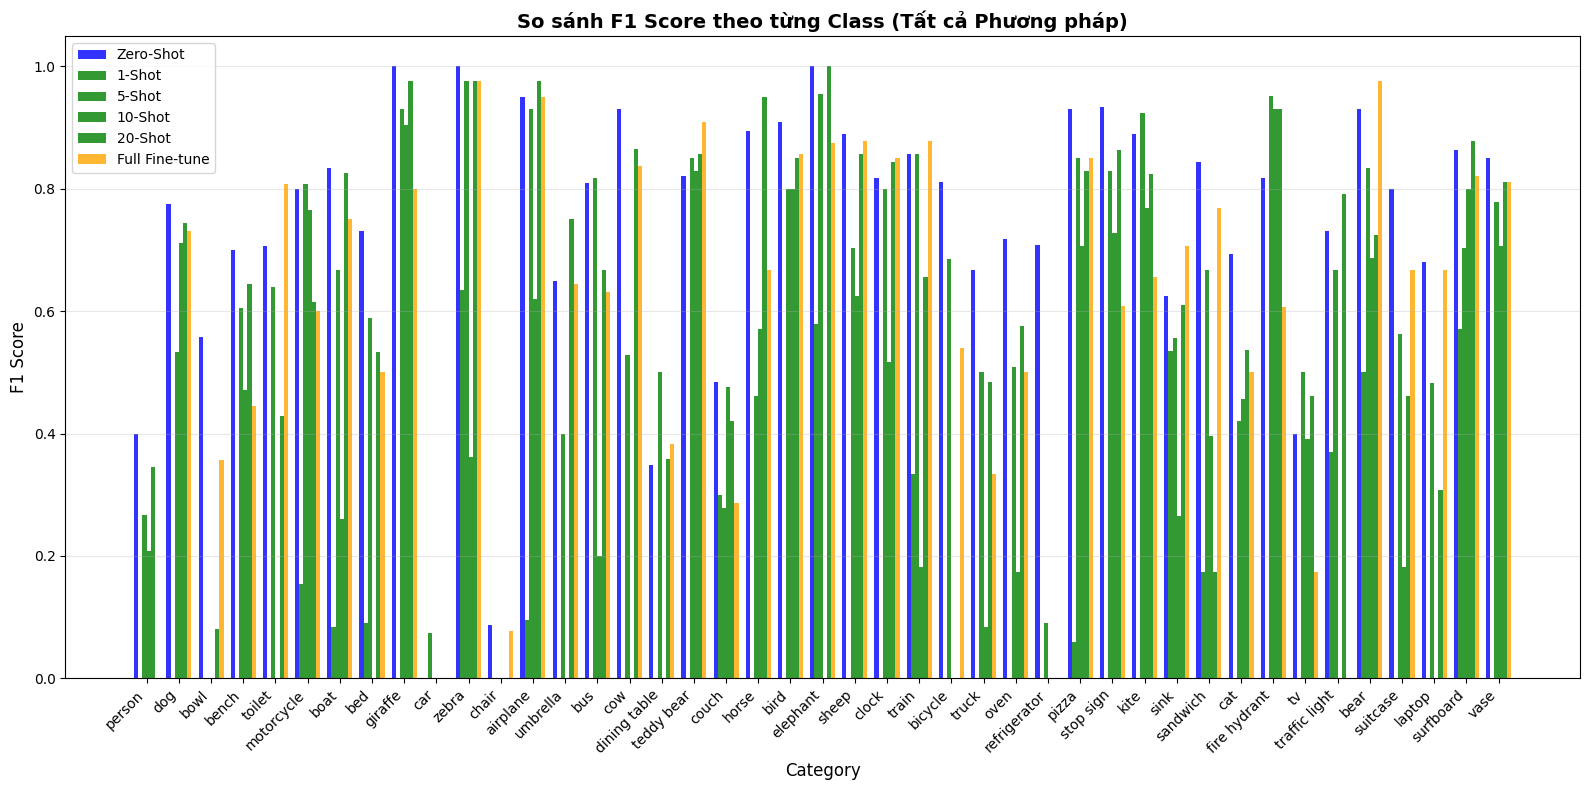
\includegraphics[width=0.95\textwidth]{Images/multimodal_per_class_f1.png}

    \vspace{0.5cm}
    \caption{So sánh F1 score theo từng category. Top performers: giraffe, zebra, elephant. Challenging: chair, person, bowl.}
    \label{fig:per-class-f1}
\end{figure}

\paragraph{Top-performing classes (F1 > 0.9)}
\begin{itemize}
    \item \textbf{giraffe}, \textbf{zebra}, \textbf{elephant}: Động vật có đặc điểm ngoại hình độc nhất
    \item \textbf{airplane}, \textbf{train}: Phương tiện lớn, dễ phân biệt
    \item \textbf{stop sign}, \textbf{pizza}: Có pattern rõ ràng
\end{itemize}

\paragraph{Challenging classes (F1 < 0.5)}
\begin{itemize}
    \item \textbf{chair}: Bị nhầm với bench, couch do cùng là đồ nội thất
    \item \textbf{person}: Xuất hiện trong nhiều context khác nhau
    \item \textbf{bowl}, \textbf{cup}: Nhỏ, khó phân biệt trong ảnh
\end{itemize}

\subsection{Kết luận}\label{subsec:conclusion}

\subsubsection{Tổng kết Kết quả}
Qua thực nghiệm so sánh ba phương pháp phân loại đa phương thức trên COCO dataset, chúng tôi rút ra các kết luận sau:

\begin{enumerate}
    \item \textbf{Zero-shot CLIP cực kỳ mạnh} cho COCO dataset (75.8\% accuracy), vượt trội hơn cả fine-tuning. Điều này chứng tỏ CLIP pretrained đã học được biểu diễn tốt cho các object categories phổ biến.

    \item \textbf{Few-shot learning hiệu quả với ít dữ liệu}. Chỉ với 5 samples/class, model đã đạt 64.5\% accuracy, cải thiện đáng kể so với 1-shot (16.2\%).

    \item \textbf{Diminishing returns khi tăng k}: Performance gần như không thay đổi từ k=5 đến k=20, cho thấy k=5 đã đủ để học được pattern cơ bản.

    \item \textbf{Hệ lụy của Full Fine-tuning trên dữ liệu nhỏ}: Việc unfreeze toàn bộ mạng backbone khổng lồ trên lượng dữ liệu ít ỏi không mang lại cải thiện. Thay vào đó, nó gây ra hiện tượng \textbf{"Quên thảm khốc" (Catastrophic Forgetting)}, khiến mô hình đánh mất năng lực tổng quát hóa nguyên bản và rơi vào trạng thái quá khớp (overfitting) cục bộ.
\end{enumerate}

\subsubsection{Trade-offs giữa các Phương pháp}

\begin{table}[H]
    \centering
    \caption{So sánh Trade-offs}
    \begin{tabular}{|l|l|l|l|}
        \hline
        \textbf{Tiêu chí} & \textbf{Zero-Shot} & \textbf{Few-Shot} & \textbf{Full Fine-tune} \\
        \hline
        Training data & Không cần & Ít (5-20/class) & Nhiều (100+/class) \\
        \hline
        Training time & 0s & Phút & Giờ \\
        \hline
        Accuracy & Tốt (75.8\%) & Khá (64.5\%) & Khá (64.4\%) \\
        \hline
        Resource cost & Thấp & Trung bình & Cao \\
        \hline
        Deployment speed & Tức thì & Nhanh & Chậm \\
        \hline
        Customization & Không & Có hạn & Toàn diện \\
        \hline
        Overfitting risk & Không có & Thấp & Cao \\
        \hline
    \end{tabular}
    \label{tab:tradeoffs}
\end{table}

\subsubsection{Khuyến nghị Sử dụng}

\paragraph{Khi nào dùng Zero-shot?}
\begin{itemize}
    \item Không có dữ liệu labeled
    \item Cần triển khai nhanh, không có thời gian training
    \item Task gần với CLIP pretraining (object recognition trên ảnh tự nhiên)
    \item Cần phân loại các classes mới liên tục
\end{itemize}

\paragraph{Khi nào dùng Few-shot (Frozen)?}
\begin{itemize}
    \item Có ít dữ liệu labeled (5-20 samples/class)
    \item Muốn cải thiện performance so với zero-shot
    \item Thời gian training giới hạn (vài phút)
    \item Muốn giữ lại generalization capability của CLIP
\end{itemize}

\paragraph{Khi nào dùng Full Fine-tuning (Unfrozen)?}
\begin{itemize}
    \item Có nhiều dữ liệu labeled (100+ samples/class)
    \item Task khác xa CLIP pretraining (medical images, satellite imagery, etc.)
    \item Có GPU và thời gian để train toàn bộ model
    \item Zero-shot và few-shot không đạt yêu cầu
\end{itemize}

\subsubsection{Hướng Phát triển}
Một số hướng cải thiện tiềm năng:
\begin{enumerate}
    \item \textbf{Prompt engineering}: Thay vì chỉ sử dụng template đơn giản \texttt{"a photo of a \{category\}"}, có thể thử các dạng prompt phong phú hơn nhằm tận dụng tối đa năng lực ngôn ngữ của CLIP để nâng cao hiệu năng Zero-shot. Ví dụ:
    \begin{itemize}
        \item \texttt{"a photo of a \{category\}, a type of animal/vehicle/object"} (cung cấp ngữ cảnh siêu phạm trù)
        \item \texttt{"a clear photo of \{category\} in natural lighting"} (mô tả điều kiện chụp)
        \item \textbf{Prompt Ensembling}: Kết hợp dự đoán từ nhiều template prompt khác nhau và lấy trung bình vector text embedding, thay vì chỉ dùng một template duy nhất. Phương pháp này được OpenAI sử dụng trong bài báo gốc của CLIP và cho thấy cải thiện đáng kể so với single-template.
    \end{itemize}
    \item \textbf{Data augmentation}: Tăng cường dữ liệu cho few-shot learning
    \item \textbf{Adapter tuning}: Thay vì full fine-tuning, chỉ thêm các adapter layers nhỏ
    \item \textbf{Knowledge distillation}: Dùng zero-shot làm teacher cho few-shot student
    \item \textbf{Ensemble methods}: Kết hợp predictions từ nhiều phương pháp
\end{enumerate}


%%%%%%%%%%%%%%%%%%%%%%%%%%%%%%%%%
% Tài liệu tham khảo
%%%%%%%%%%%%%%%%%%%%%%%%%%%%%%%%%
\addcontentsline{toc}{section}{Tài liệu tham khảo}
\begin{thebibliography}{99999}
	\bibitem{radford2021learning}
	Radford, A., Kim, J. W., Hallacy, C., Ramesh, A., Goh, G., Agarwal, S., ... \& Sutskever, I. (2021).
		{\em Learning transferable visual models from natural language supervision.}
	In International Conference on Machine Learning (pp. 8748-8763). PMLR.

	\bibitem{lin2014microsoft}
	Lin, T. Y., Maire, M., Belongie, S., Hays, J., Perona, P., Ramanan, D., ... \& Zitnick, C. L. (2014).
		{\em Microsoft COCO: Common objects in context.}
	In European conference on computer vision (pp. 740-755). Springer, Cham.

	\bibitem{snell2017prototypical}
	Snell, J., Swersky, K., \& Zemel, R. (2017).
		{\em Prototypical networks for few-shot learning.}
	Advances in neural information processing systems, 30.

	% 	\bibitem[Dal]{Dal}{Dalgaard, P.} {\em Introductory Statistics with R.}  Springer 2008.

	% 	\bibitem[K-Z]{K-Z}{Kenett, R. S. and Zacks, S.}
	% 	{\em Modern Industrial Statistics: with applications in R, MINITAB and JMP,} 2nd ed.,  John Wiley and Sons, 2014.

	% 	\bibitem[Ker]{Ker}{Kerns, G. J.}
	% 	{\em Introduction to Probability and Statistics Using R,} 2nd ed., CRC 2015.

\end{thebibliography}
\end{document}